\documentclass[12pt, a4paper]{article}
\usepackage[margin = 1in, top=1.3in]{geometry}
\usepackage[english]{babel}
\usepackage[utf8]{inputenc}
\usepackage{fancyhdr}
\usepackage{amsmath}
\usepackage{bm}
\usepackage{float}
\usepackage{graphicx}
\usepackage[font=small,labelfont=bf]{caption}

\graphicspath{{./images/}}
 
\pagestyle{fancy}
\fancyhf{}
\rhead{\small{Shaan Ul Haque(180070053)\\ Samarth Singh (180050090) \\ Niraj Mahajan (180050069)}}
\lhead{CS-663 Assignment-1 : Question 2}
% \rfoot{Page i.\thepage}
 
\begin{document}
\vspace*{-22pt}
\section*{Question 2}
\subsection*{Part A : Foreground Mask (2 points)}
%\vspace*{-40pt}
\begin{figure}[H]
    \centering
%    \vspace*{-30pt}
    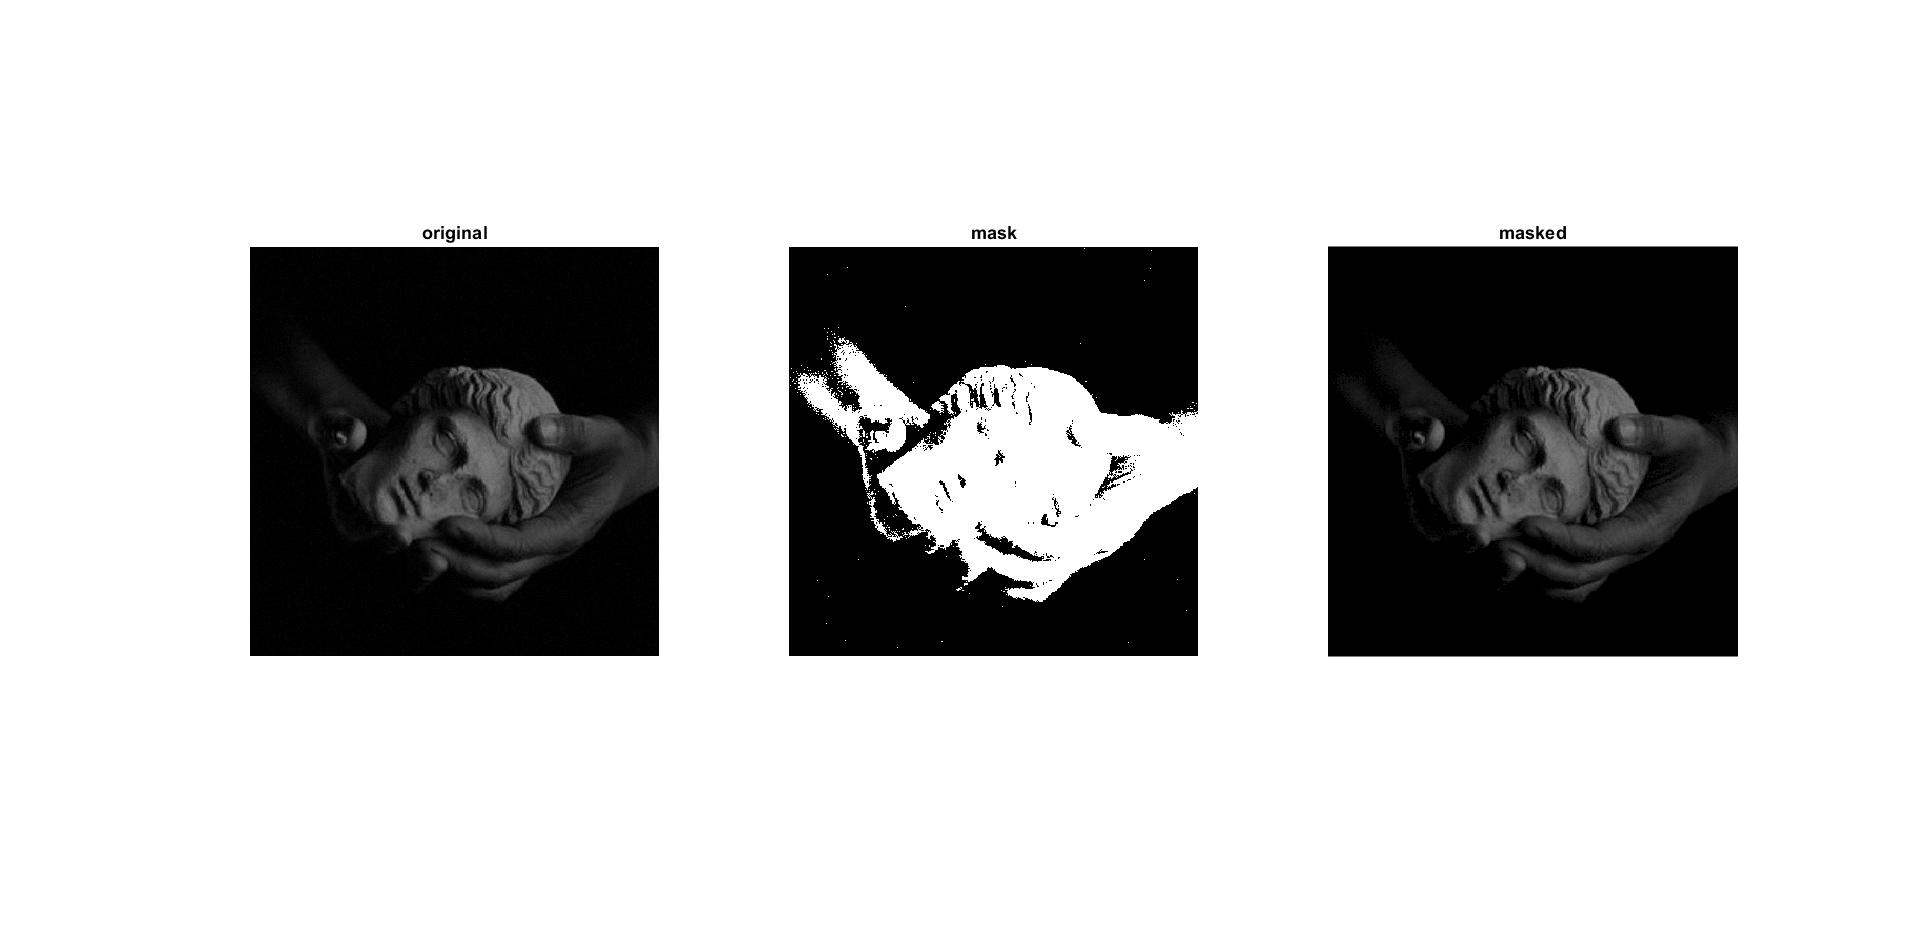
\includegraphics[width=\textwidth]{a7.jpg}
    \vspace*{-70pt}
    \caption{Transformation on Image(7)}
    \label{}
\end{figure}

\subsection*{Part B : Linear Contrast Stretching (3 points)}
Formula used :- \\
 $$ {F(x) = a + ((x-a)/(b-a))*255} $$
where,\\
\begin{itemize}
\vspace{-0.8 cm}
    \item a is the intensity with 5 percentile (w.r.t. intensities sorted in ascending order)
\vspace{-0.4 cm}
    \item b is the intensity with 95 percentile (w.r.t. intensities sorted in ascending order)
\end{itemize}
\textbf{Observations after applying on Image(5)} :-\\
Application of Contrast stretching on image(5) doesn't create any significant visible change in the image. \\
\textbf{Reason} :- \\
The image already had a complete intensity range, so linear contrast stretching won't be effective as according the formula (b-a) tends to 255 so the intensities will be mapped to the same value. \\  

\renewcommand{\thefigure}{2.1}
\begin{figure}[H]
    \centering
%    \vspace*{-30pt}
    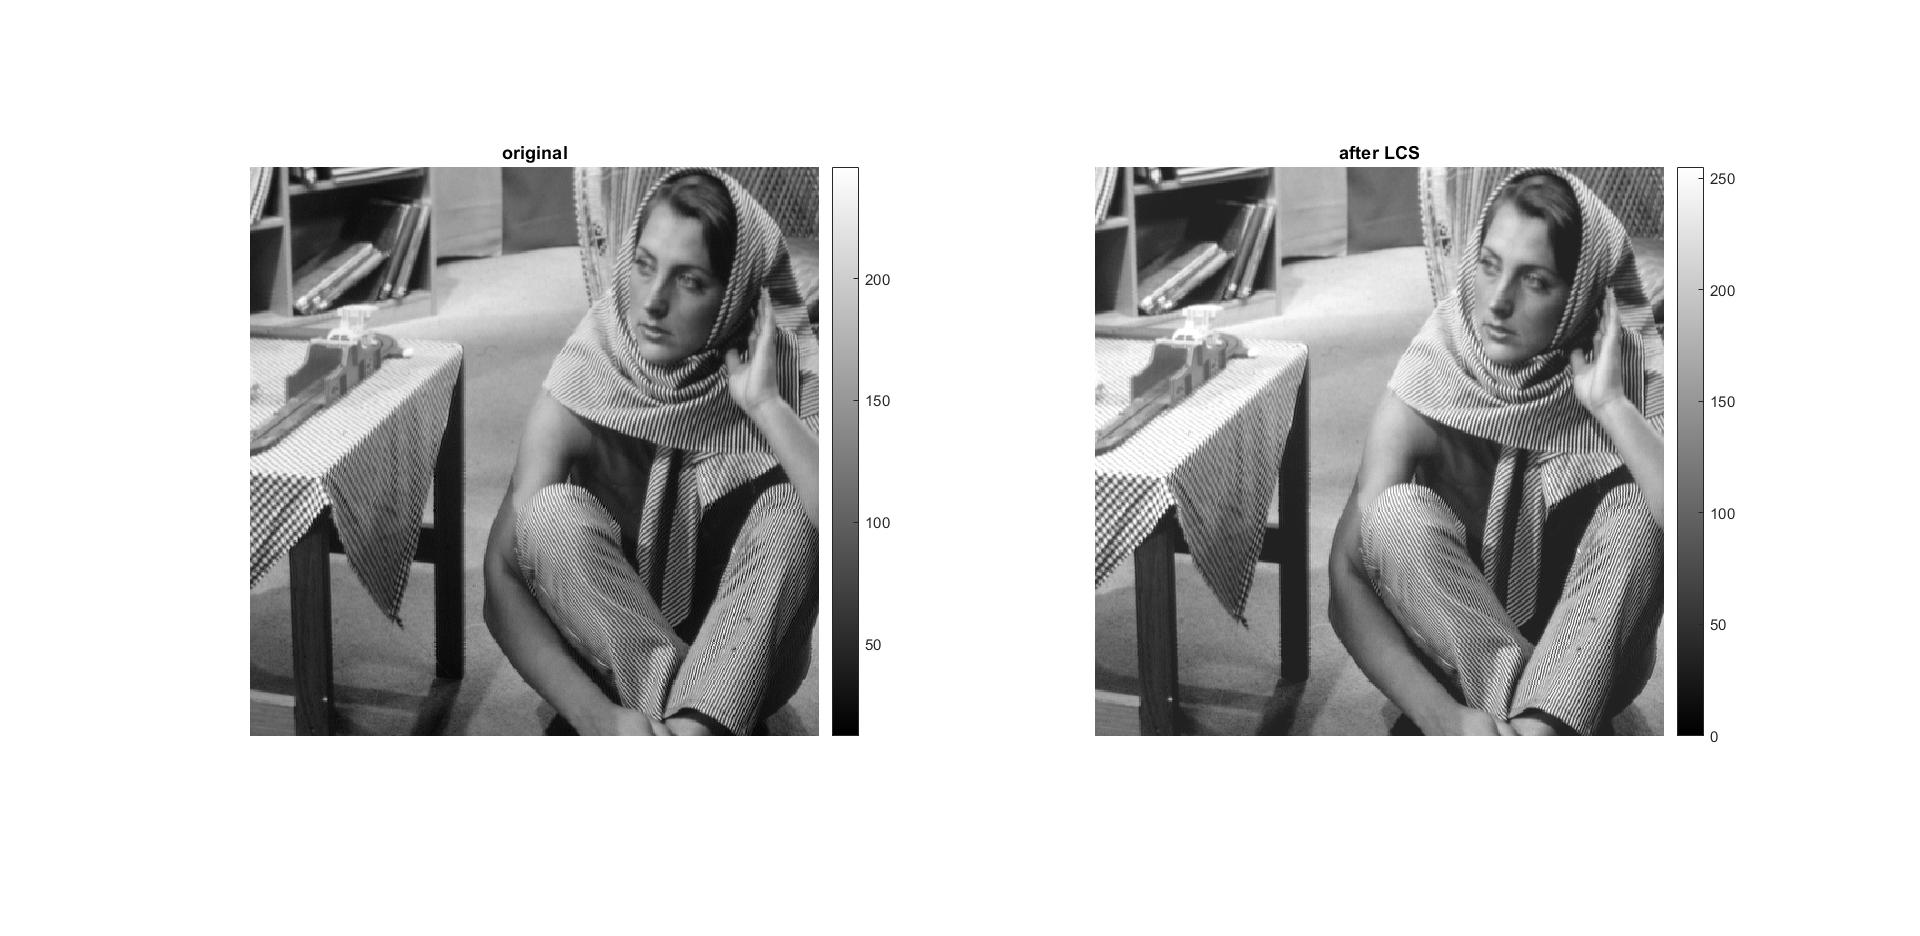
\includegraphics[width=\textwidth]{b1.jpg}
    \vspace*{-55pt}
    \caption{Transformation on Image(1)}
    \label{fig:2.1}
\end{figure}
\renewcommand{\thefigure}{2.2}
\begin{figure}[H]
    \centering
    \vspace*{-30pt}
    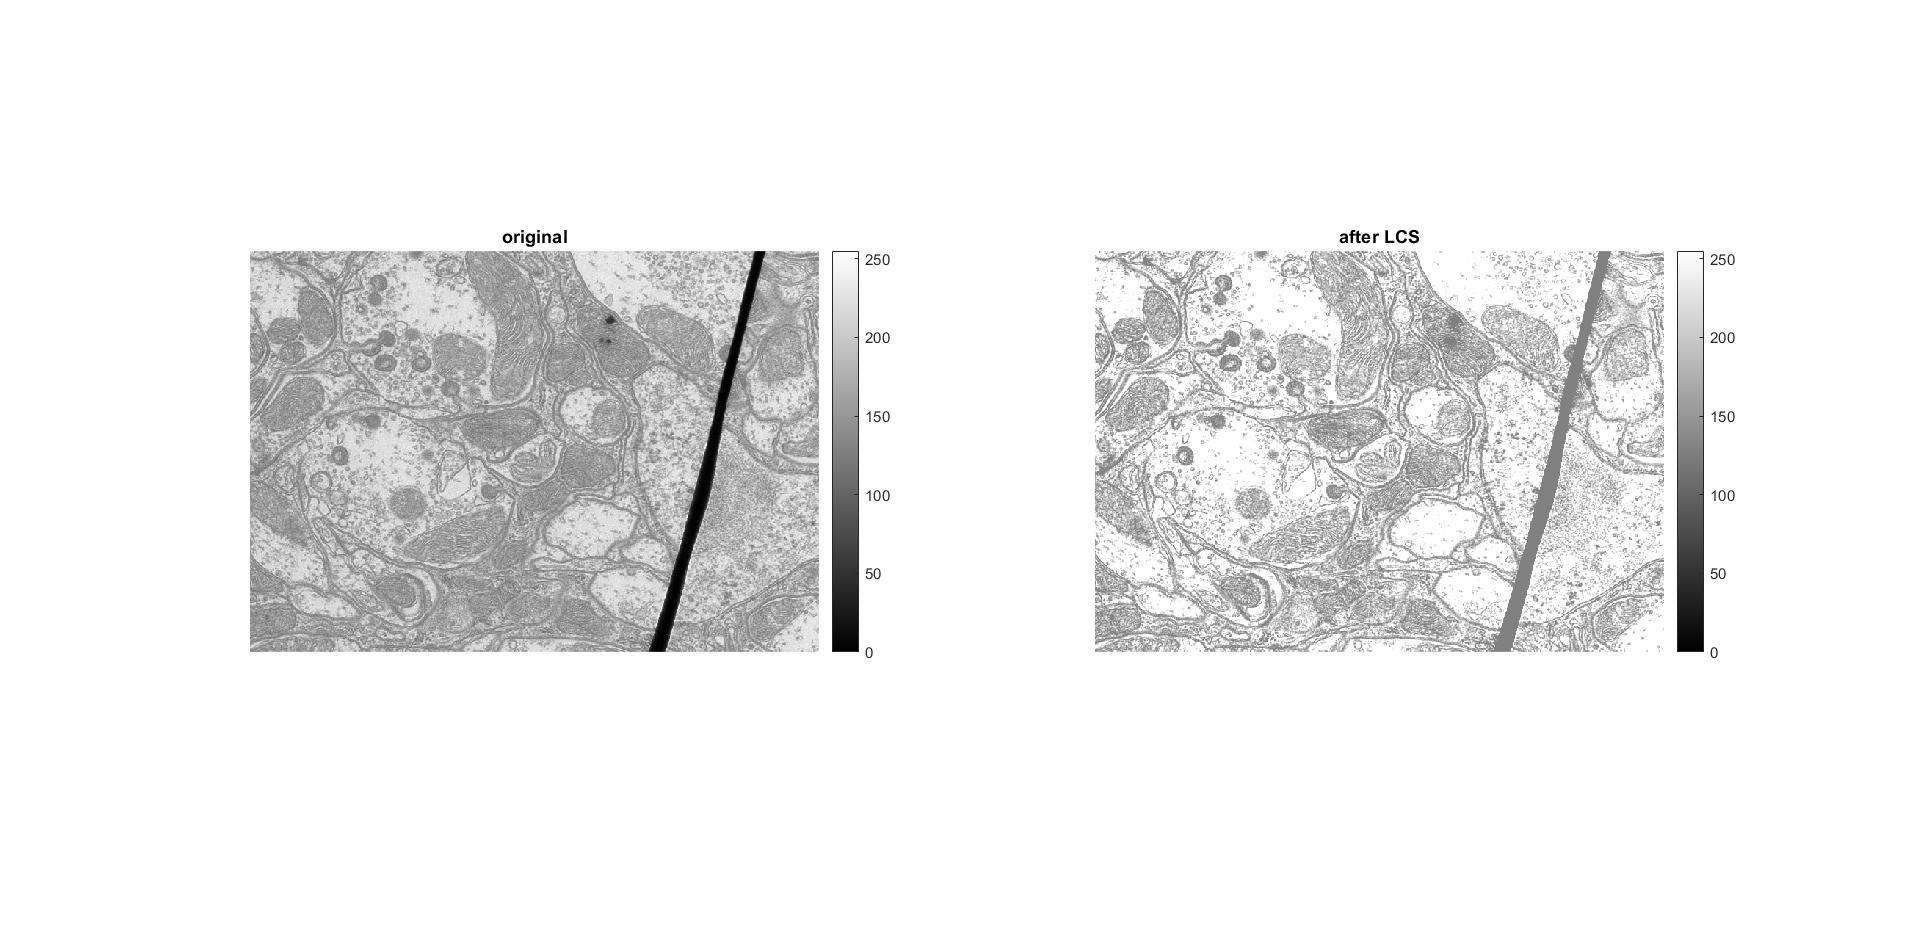
\includegraphics[width=\textwidth]{b2.jpg}
    \vspace*{-70pt}
    \caption{Transformation on Image(2)}
    \label{fig:2.2}
\end{figure}
\renewcommand{\thefigure}{2.3}
\begin{figure}[H]
    \centering
    \vspace*{-30pt}
    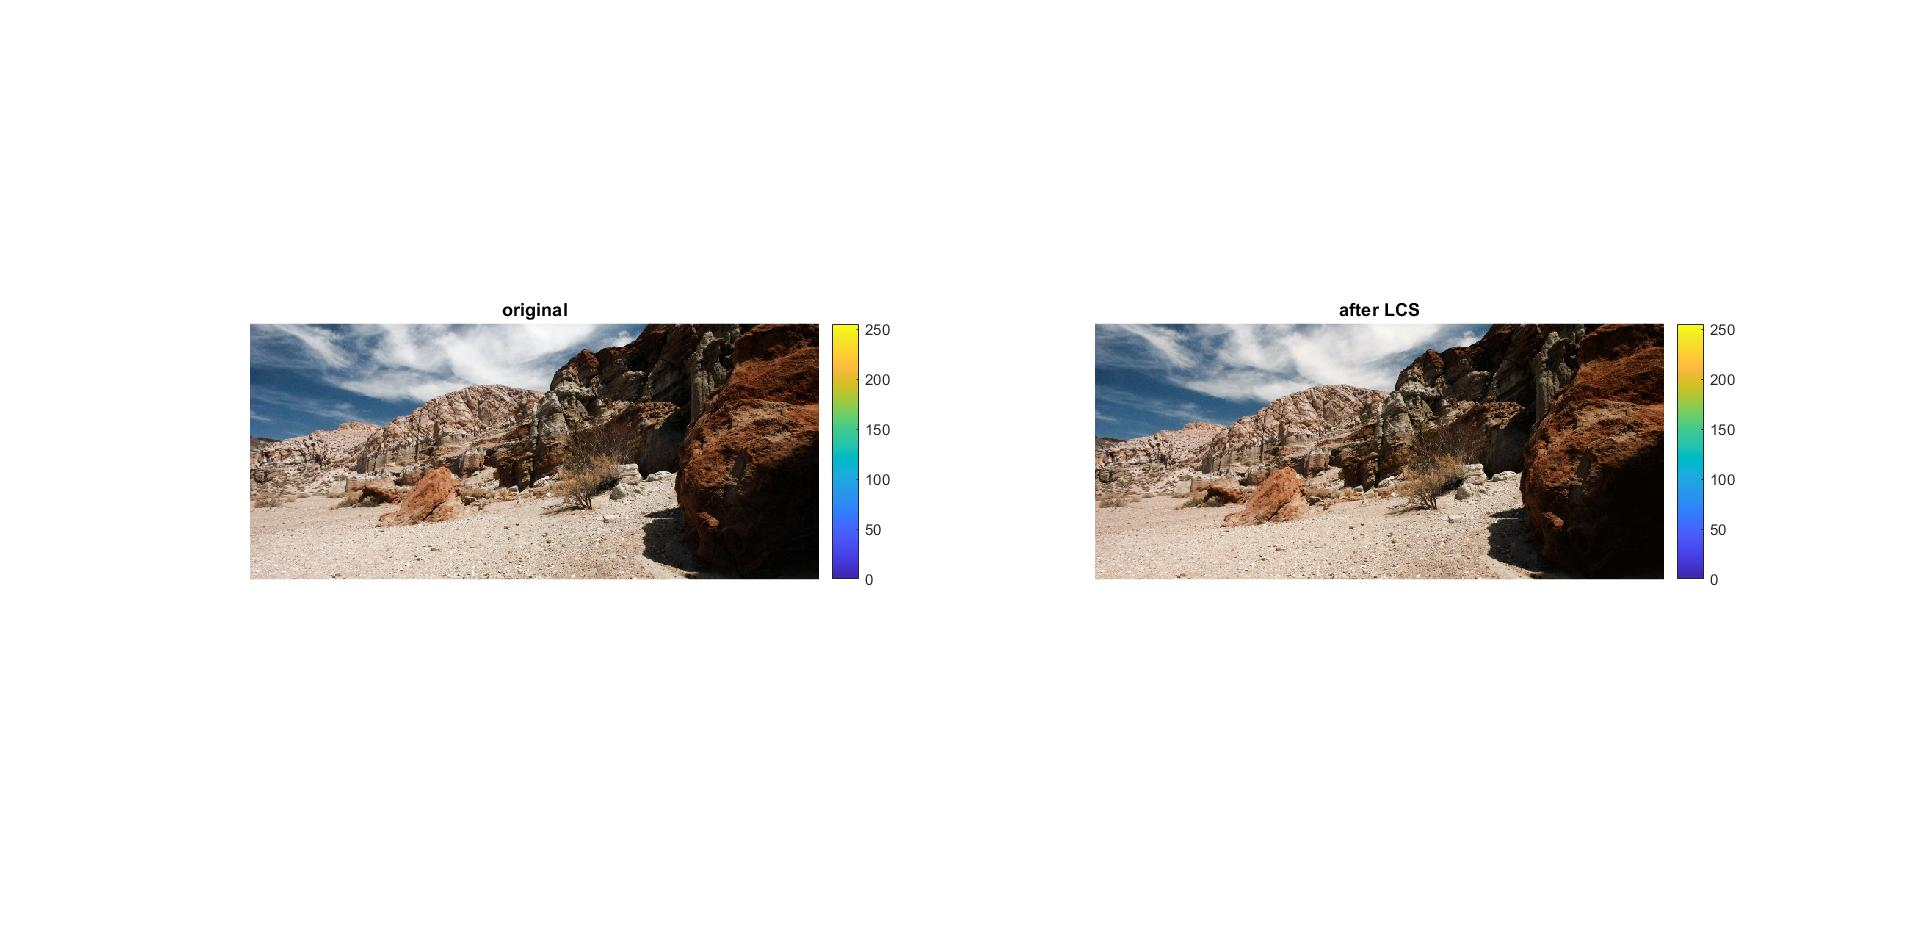
\includegraphics[width=\textwidth]{b3.jpg}
    \vspace*{-90pt}
    \caption{Transformation on Image(3)}
    \label{fig:2.3}
\end{figure}
\newpage
\renewcommand{\thefigure}{2.5}
\begin{figure}[H]
    \centering
%    \vspace*{-30pt}
    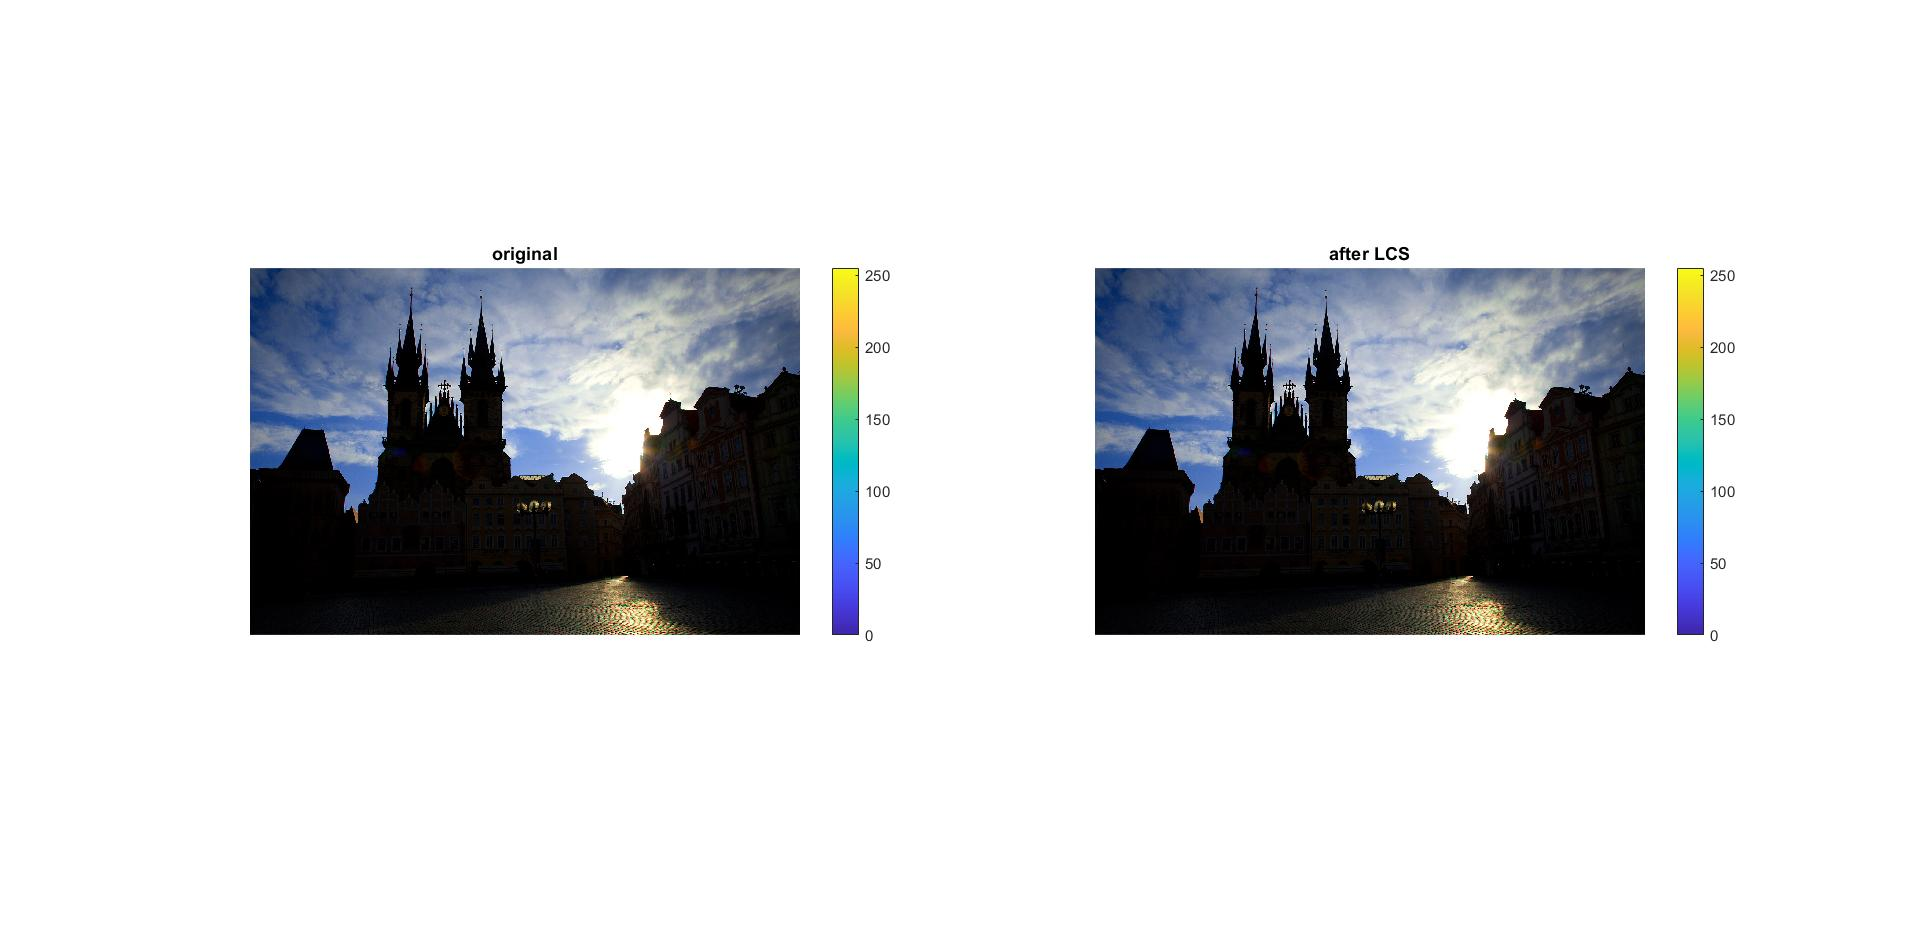
\includegraphics[width=\textwidth]{b5.jpg}
    \vspace*{-75pt}
    \caption{Transformation on Image(5)}
    \label{fig:2.5}
\end{figure}
\renewcommand{\thefigure}{2.6}
\begin{figure}[H]
    \centering
    \vspace*{-30pt}
    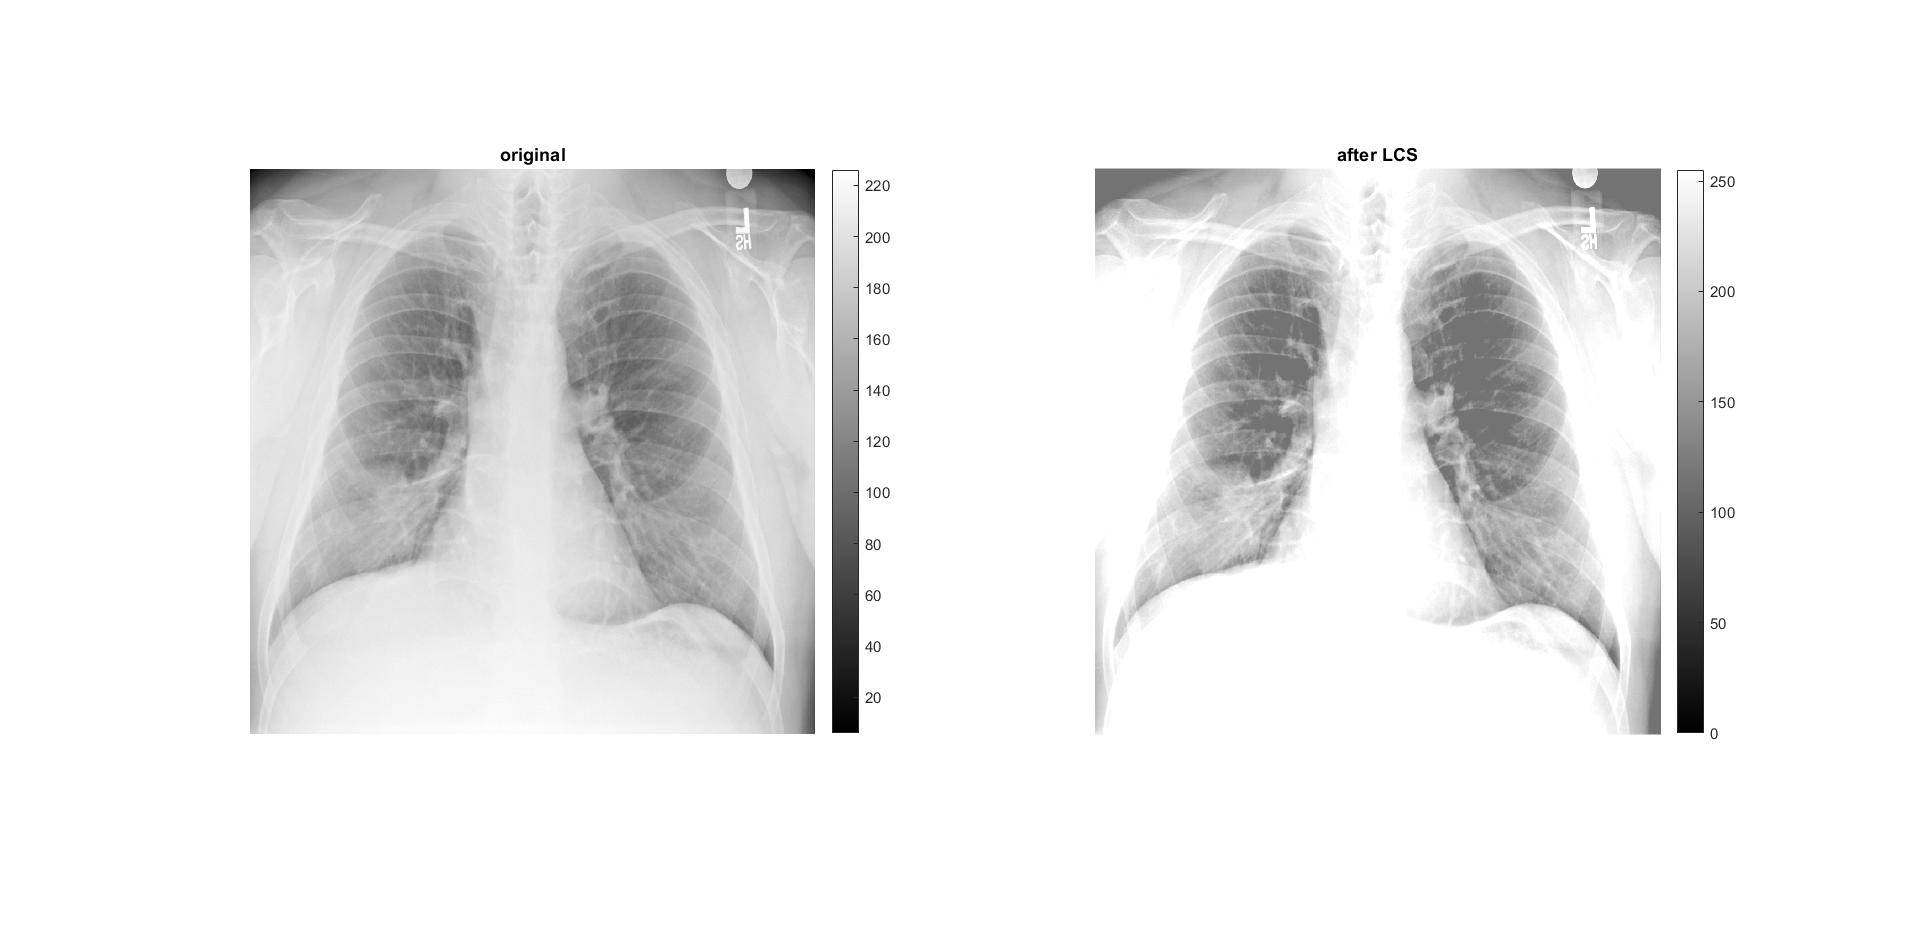
\includegraphics[width=\textwidth]{b6.jpg}
    \vspace*{-50pt}
    \caption{Transformation on Image(6)}
    \label{fig:2.6}
\end{figure}
\renewcommand{\thefigure}{2.7}
\begin{figure}[H]
    \centering
    \vspace*{-30pt}
    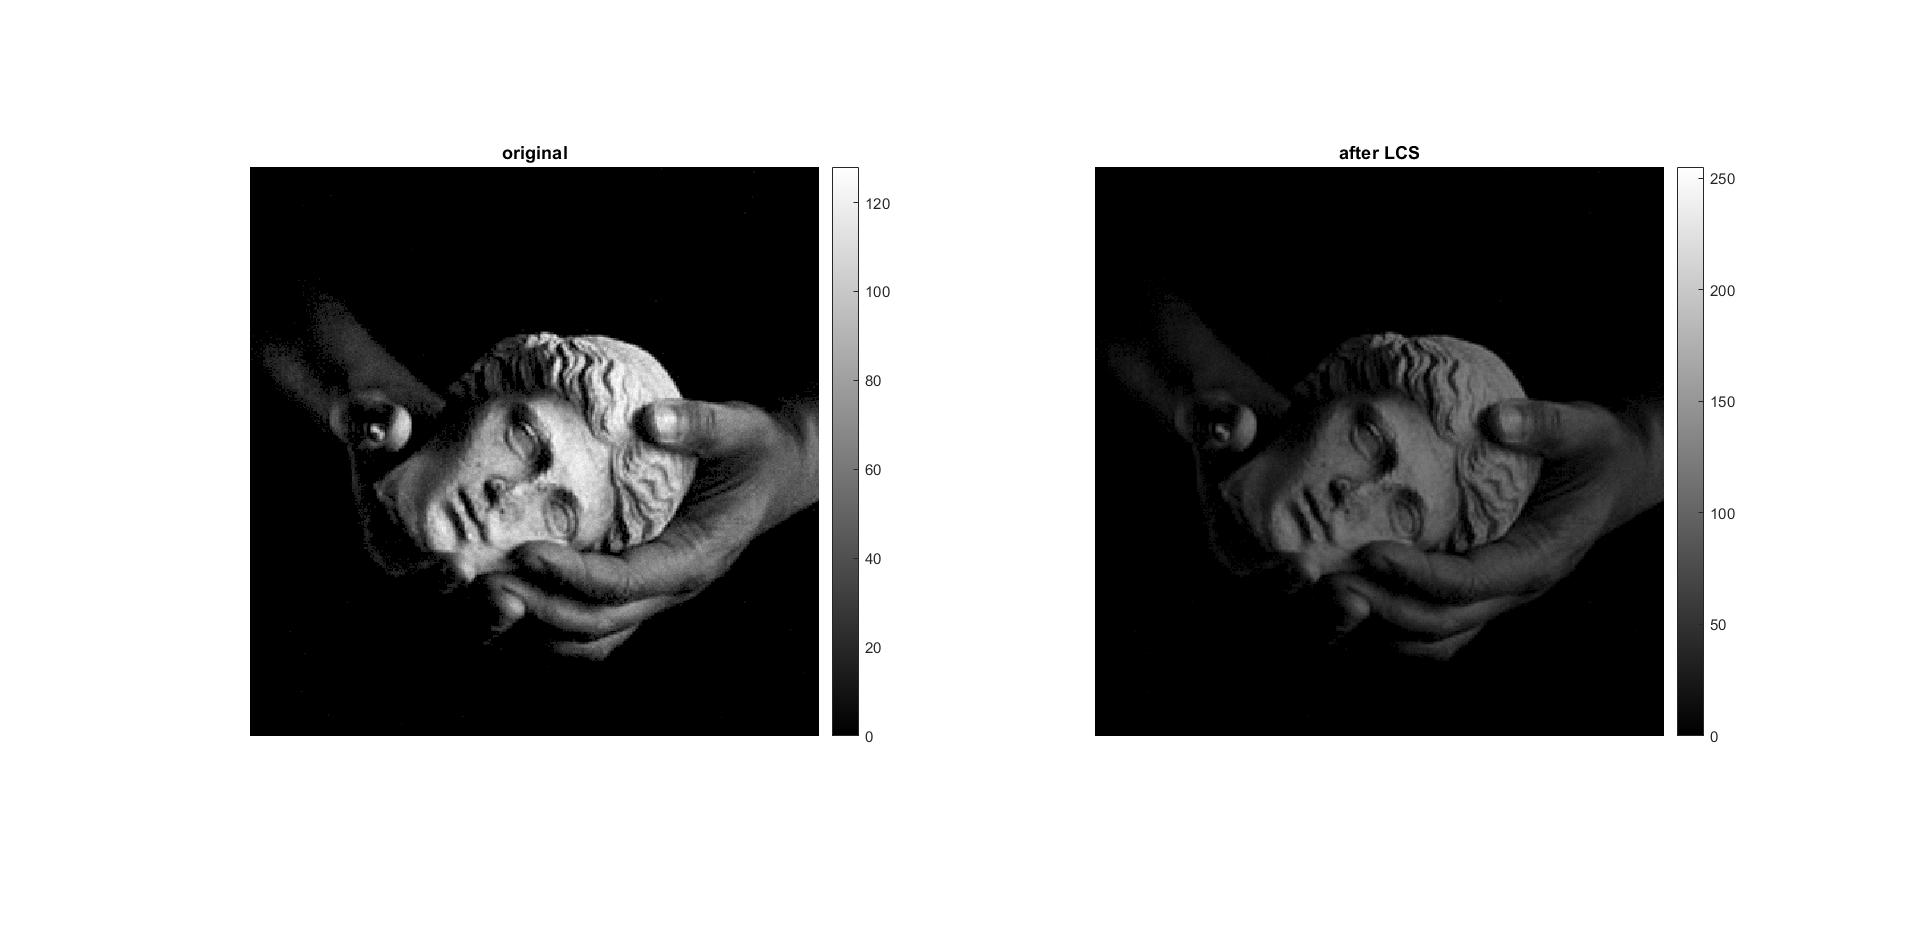
\includegraphics[width=\textwidth]{b7.jpg}
    \vspace*{-60pt}
    \caption{Transformation on Image(7) \\Please note the image on the left is after LCS, while the one on the right is orignal}
    \label{fig:2.7}
\end{figure}
\newpage
\subsection*{Part C : Histogram Equalization (HE) (5 points)}
\textbf{Observations after applying on Image(5)} :- \\
Application of Histogram Equalization on Image(5) results in a significant improvement in the image quality. Thus, we should prefer HE over linear contrast stretching. \\
\textbf{Reason} :- \\
The Image(5) had a higher frequency of lower intensities, and after HE, the equalized intensities resulted in a much better image. \\
%insert images with name starting with c
%write caption like transformation of image(x) where x is the no. following c in image name

\renewcommand{\thefigure}{3.1}
\begin{figure}[H]
    \centering
%    \vspace*{-30pt}
    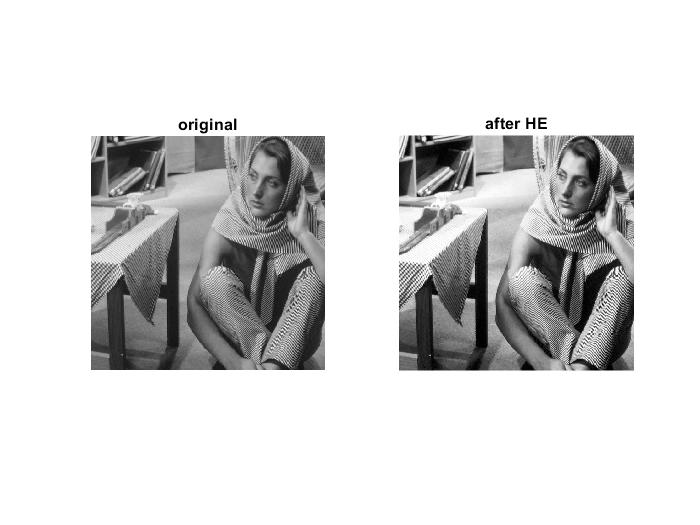
\includegraphics[width=\textwidth]{c1.jpg}
    \vspace*{-110pt}
    \caption{Transformation on Image(1)}
    \label{fig:3.1}
\end{figure}
\renewcommand{\thefigure}{3.2}
\begin{figure}[H]
    \centering
    \vspace*{-30pt}
    \vspace*{-2.5pt}
    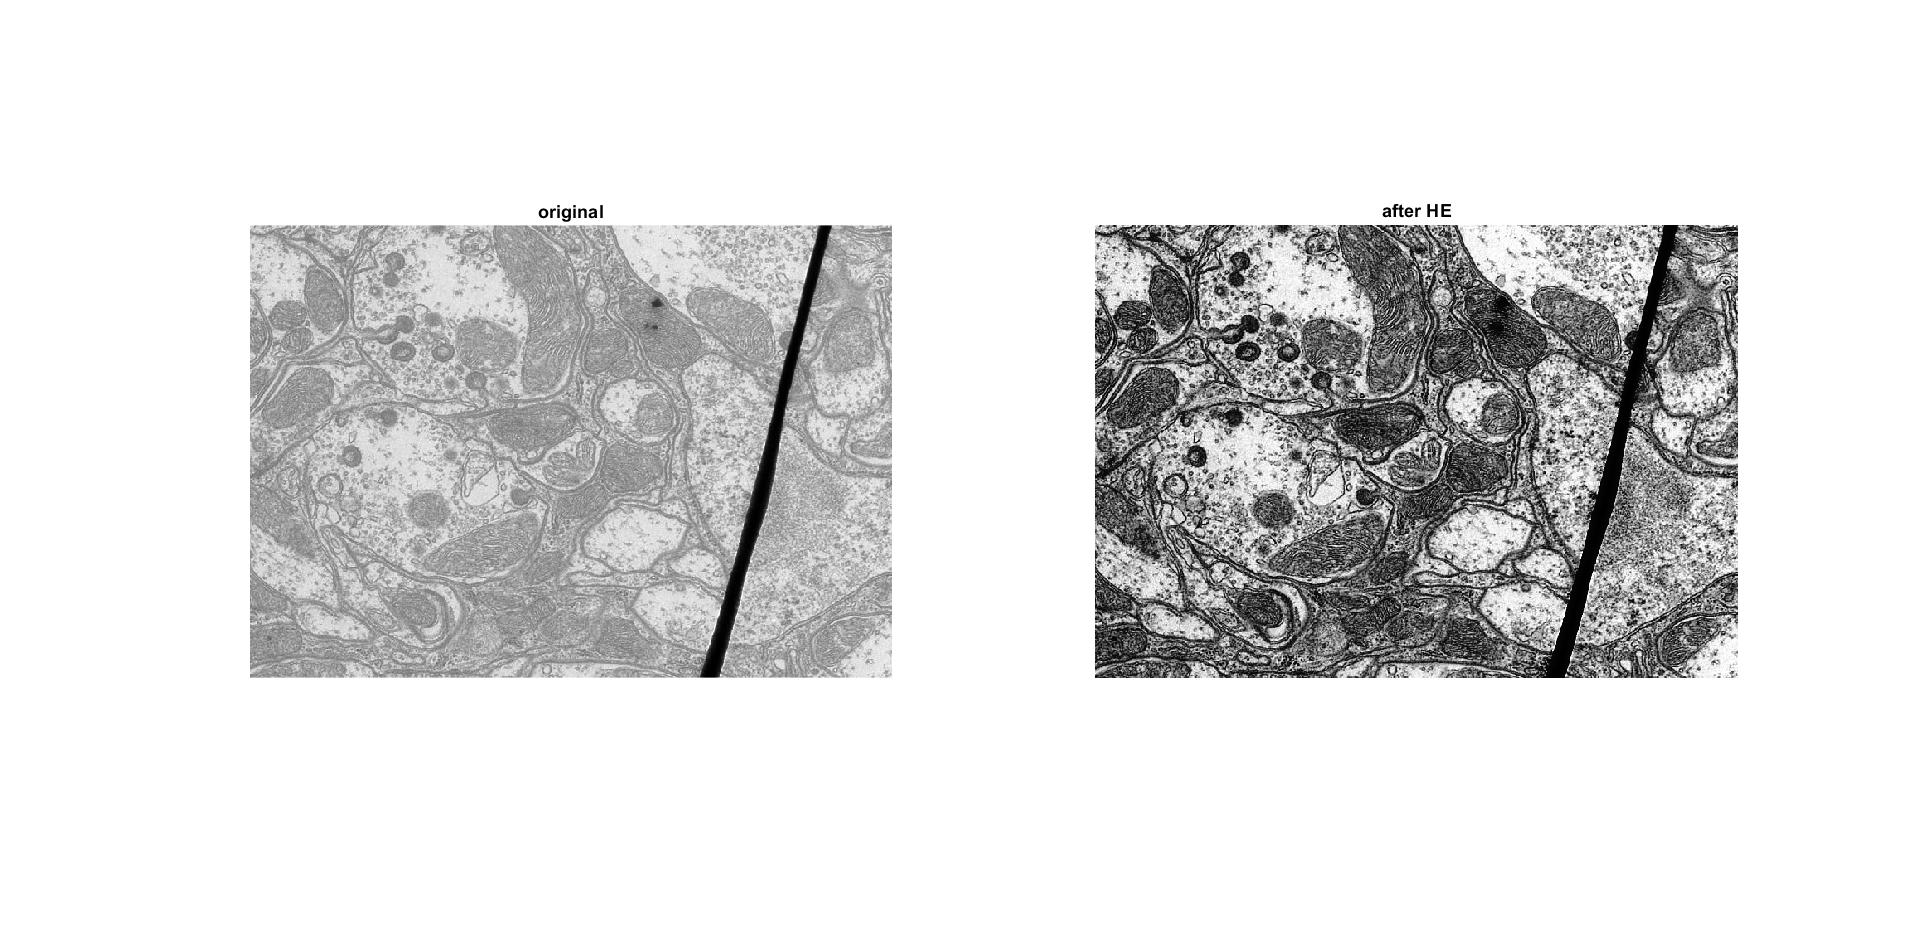
\includegraphics[width=\textwidth]{c2.jpg}
    \vspace*{-70pt}
    \caption{Transformation on Image(2)}
    \label{fig:3.2}
\end{figure}
\newpage
\renewcommand{\thefigure}{3.3}
\begin{figure}[H]
    \centering
%    \vspace*{-30pt}
    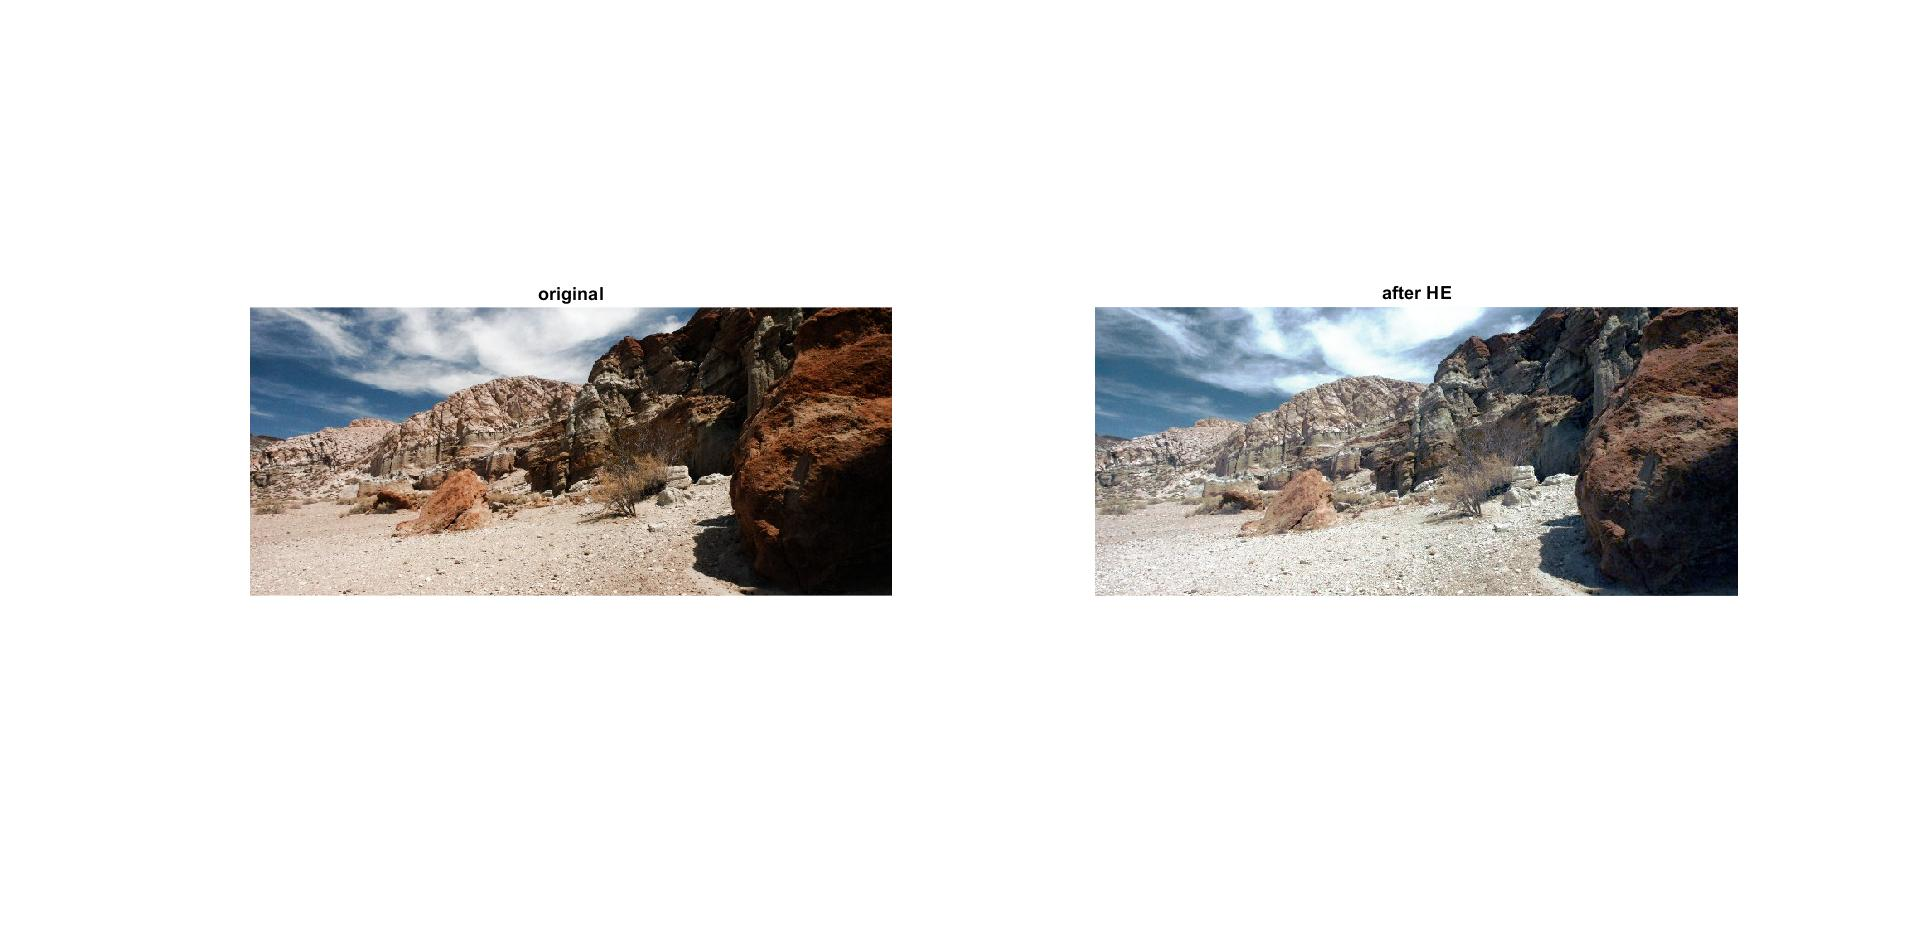
\includegraphics[width=\textwidth]{c3.jpg}
    \vspace*{-90pt}
    \caption{Transformation on Image(3)}
    \label{fig:3.3}
\end{figure}
\renewcommand{\thefigure}{3.5}
\begin{figure}[H]
    \centering
    \vspace*{-30pt}
    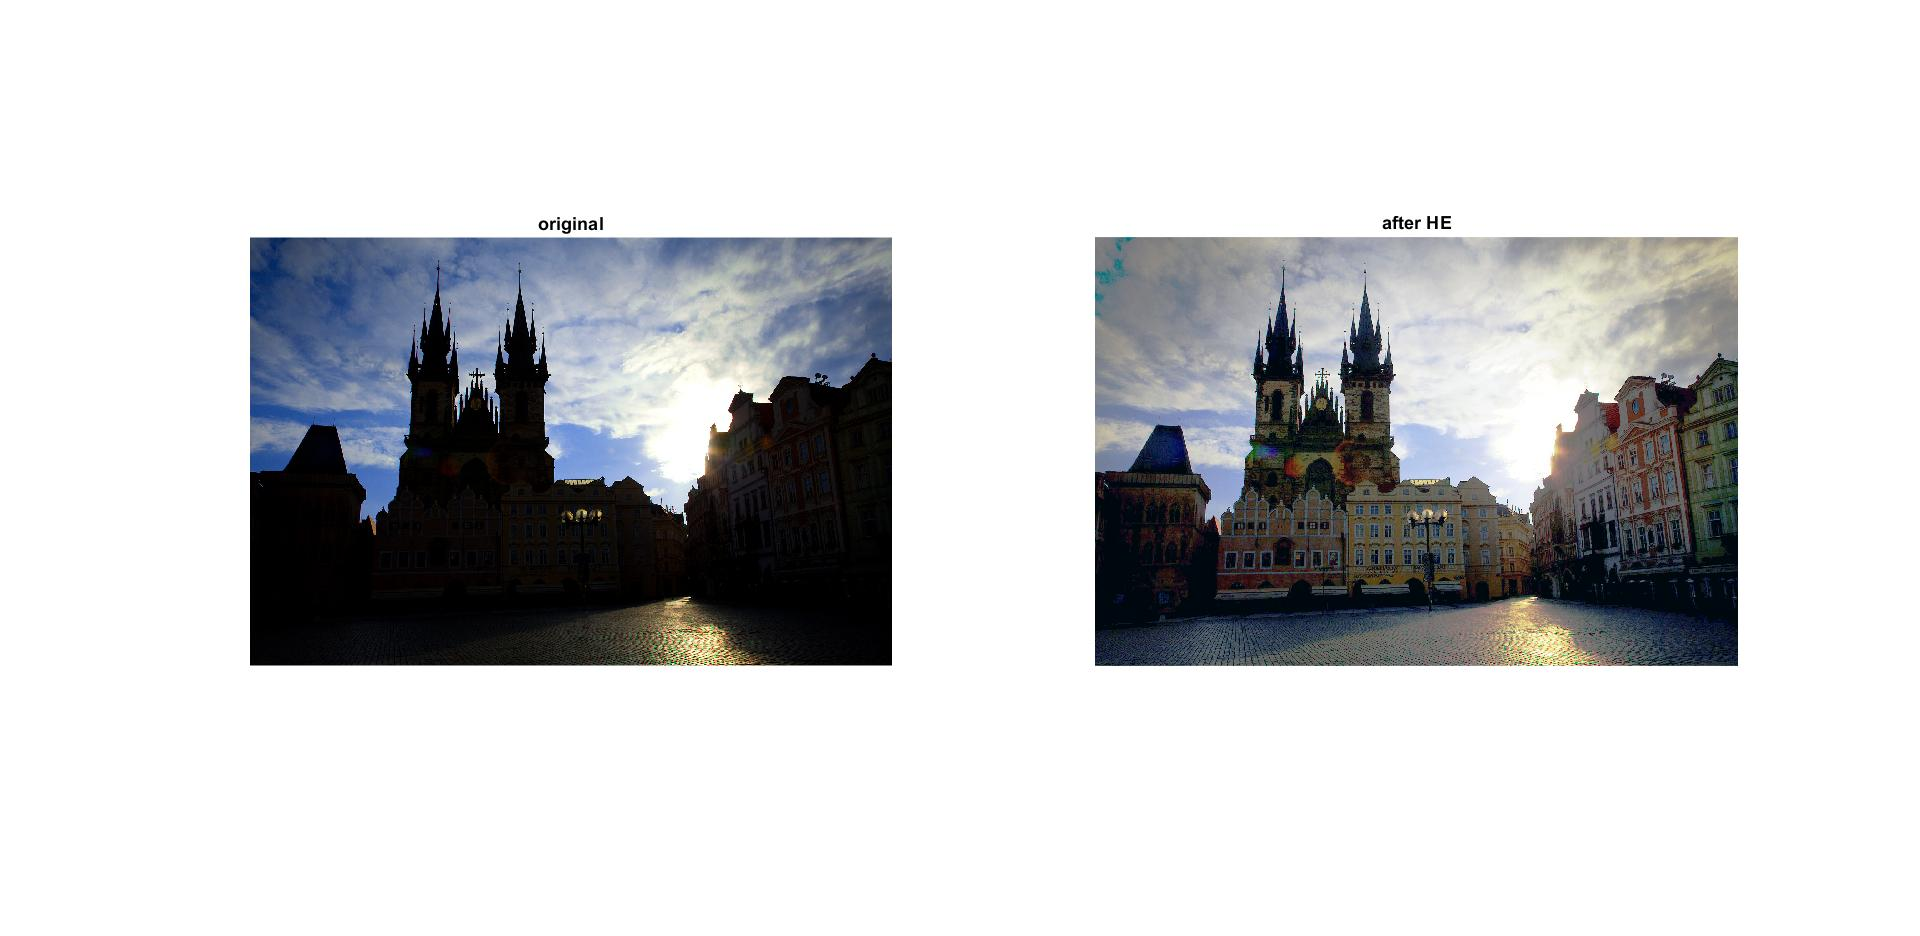
\includegraphics[width=\textwidth]{c5.jpg}
    \vspace*{-75pt}
    \caption{Transformation on Image(5)}
    \label{fig:3.5}
\end{figure}
\renewcommand{\thefigure}{3.6}
\begin{figure}[H]
    \centering
    \vspace*{-30pt}
    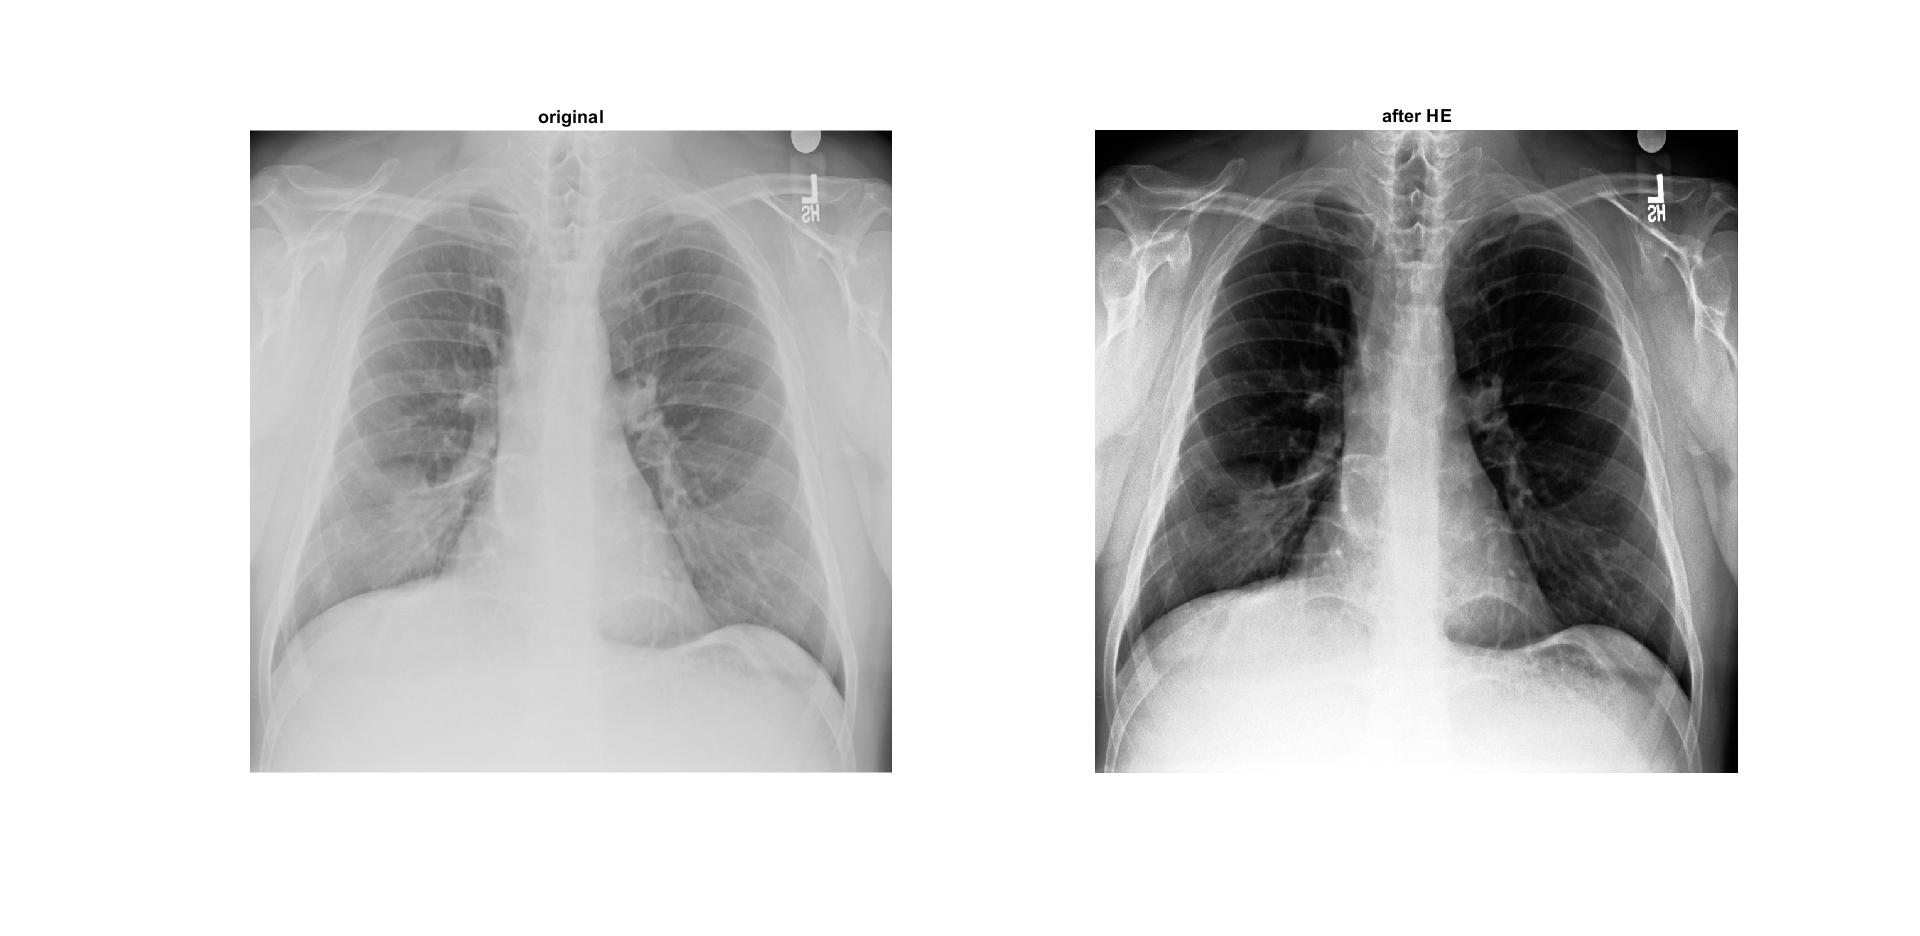
\includegraphics[width=\textwidth]{c6.jpg}
    \vspace*{-50pt}
    \caption{Transformation on Image(6)}
    \label{fig:3.6}
\end{figure}
\renewcommand{\thefigure}{3.7}
\begin{figure}[H]
    \centering
%    \vspace*{-30pt}
    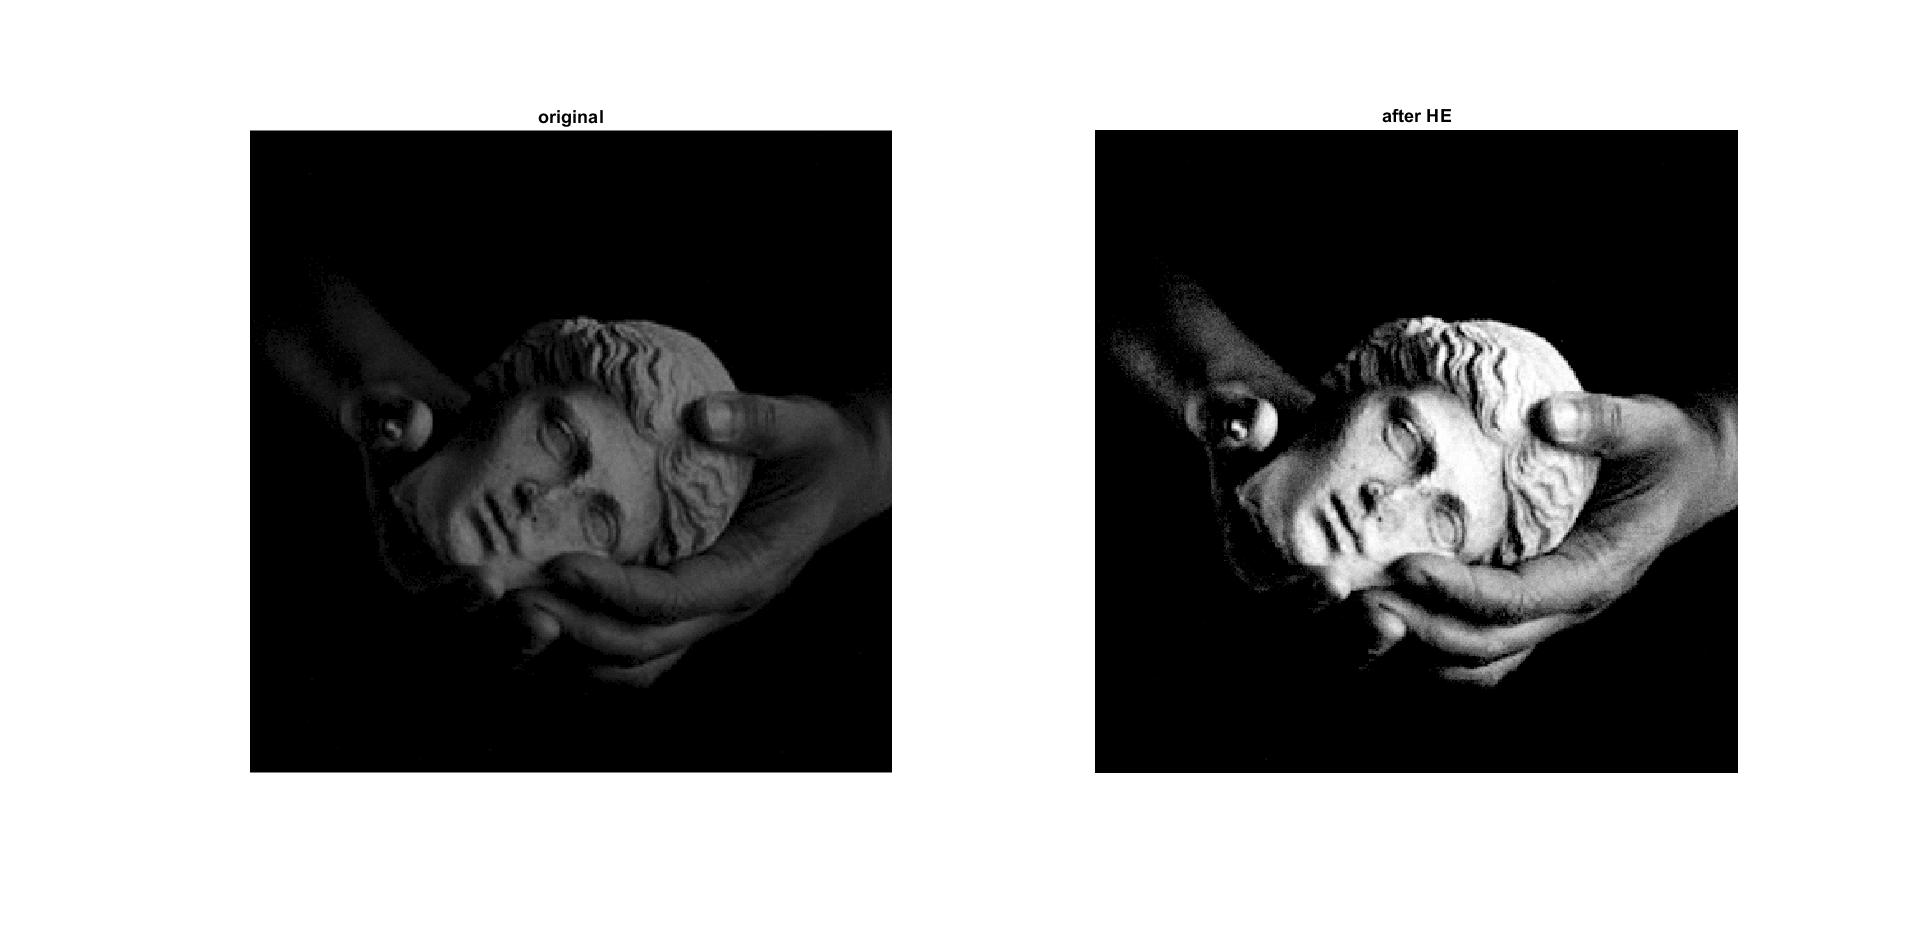
\includegraphics[width=\textwidth]{c7.jpg}
    \vspace*{-50pt}
    \caption{Transformation on Image(7)}
    \label{fig:3.7}
\end{figure}

\subsection*{Part D : Histogram Matching (HM) (15 points)}
\textbf{Observations} :- It can be observed from the above 3 images that the output of Histogram Matching is quite similar to the input image (the orange tint), while the output of HE has far more blood vessels highlighted and clearly visible.
 \\
\textbf{Reason} :- Histogram Matching is basically "enhancing" the input image while constraining the features of the output to a particular reference image. Hence, although the HE output has a lot more blood vessels visible, the HM output is quite similar in appearance to the input image, and hence more realistic. This is particulary useful when we want to enhnace the features in an image, while making it look like similar to a reference image.
 \\
\renewcommand{\thefigure}{4.1}
\begin{figure}[H]
    \centering
%    \vspace*{-30pt}
    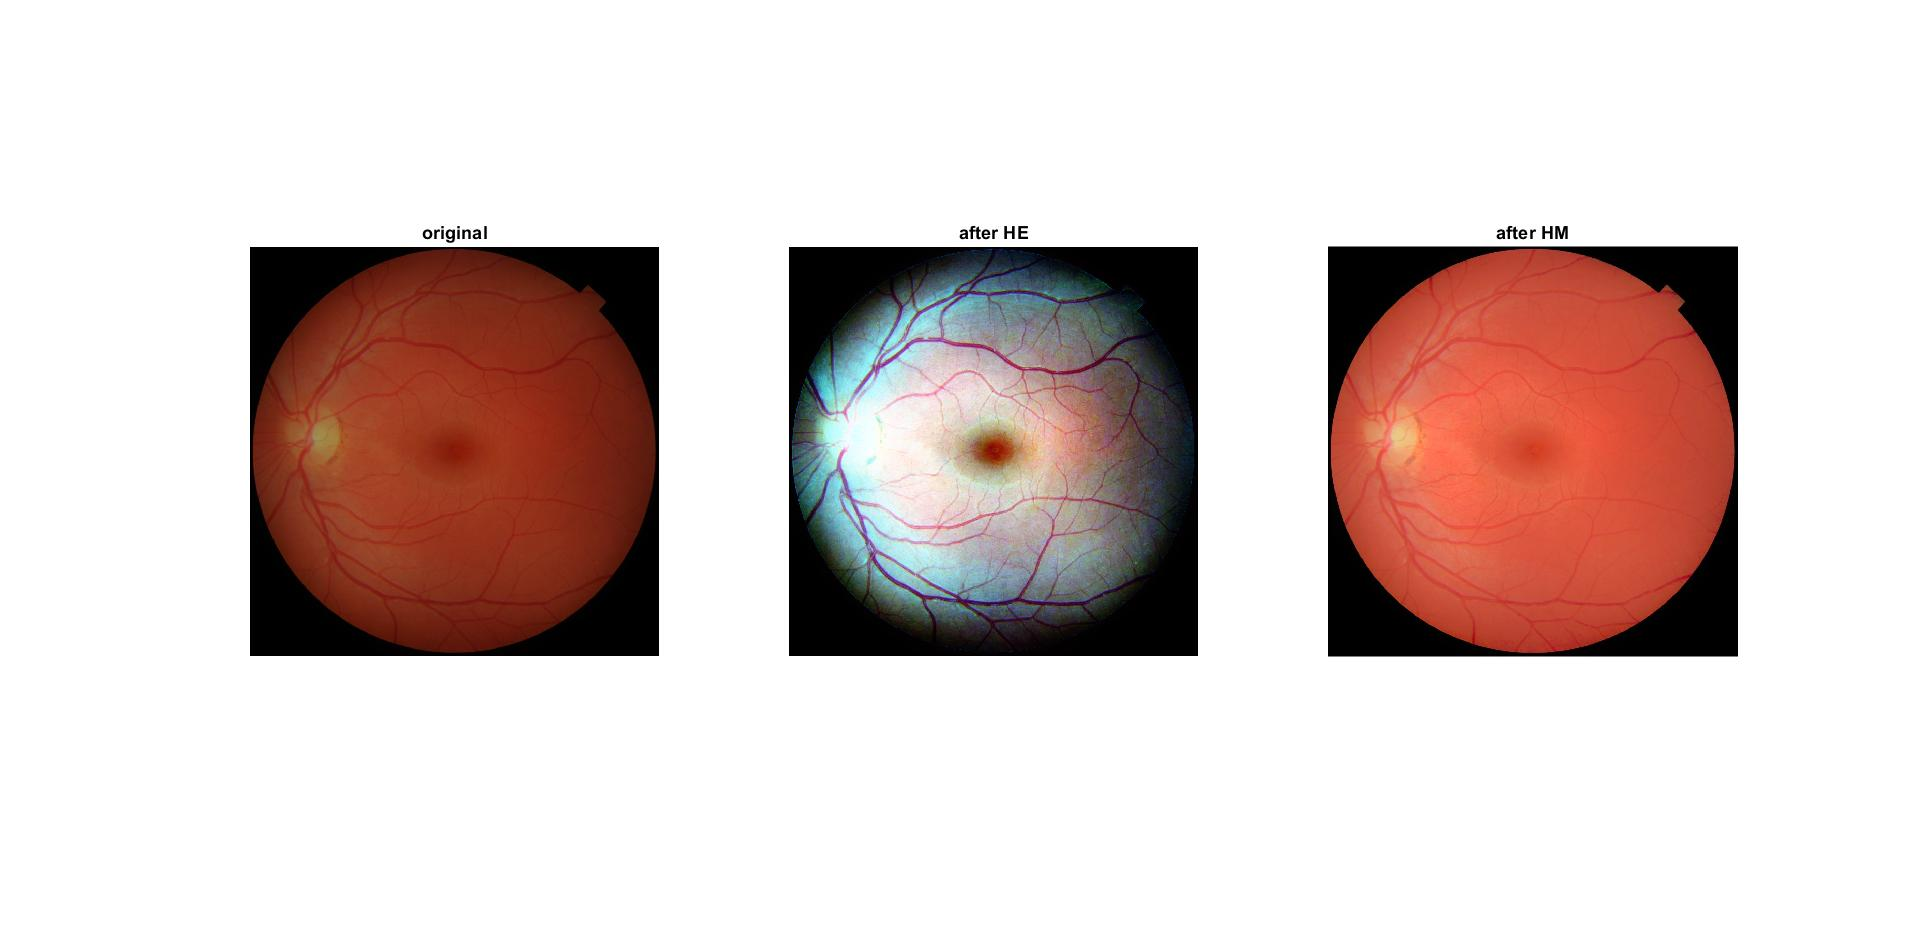
\includegraphics[width=\textwidth]{d4.jpg}
    \vspace*{-80pt}
    \caption{Transformation on Image(4)}
    \label{fig:4.1}
\end{figure}

\subsection*{Part E :  Contrast-Limited Adaptive Histogram Equalization (CLAHE) 
(30 points)}

\renewcommand{\thefigure}{5.11}
\begin{figure}[H]
    \centering
%    \vspace*{-30pt}
    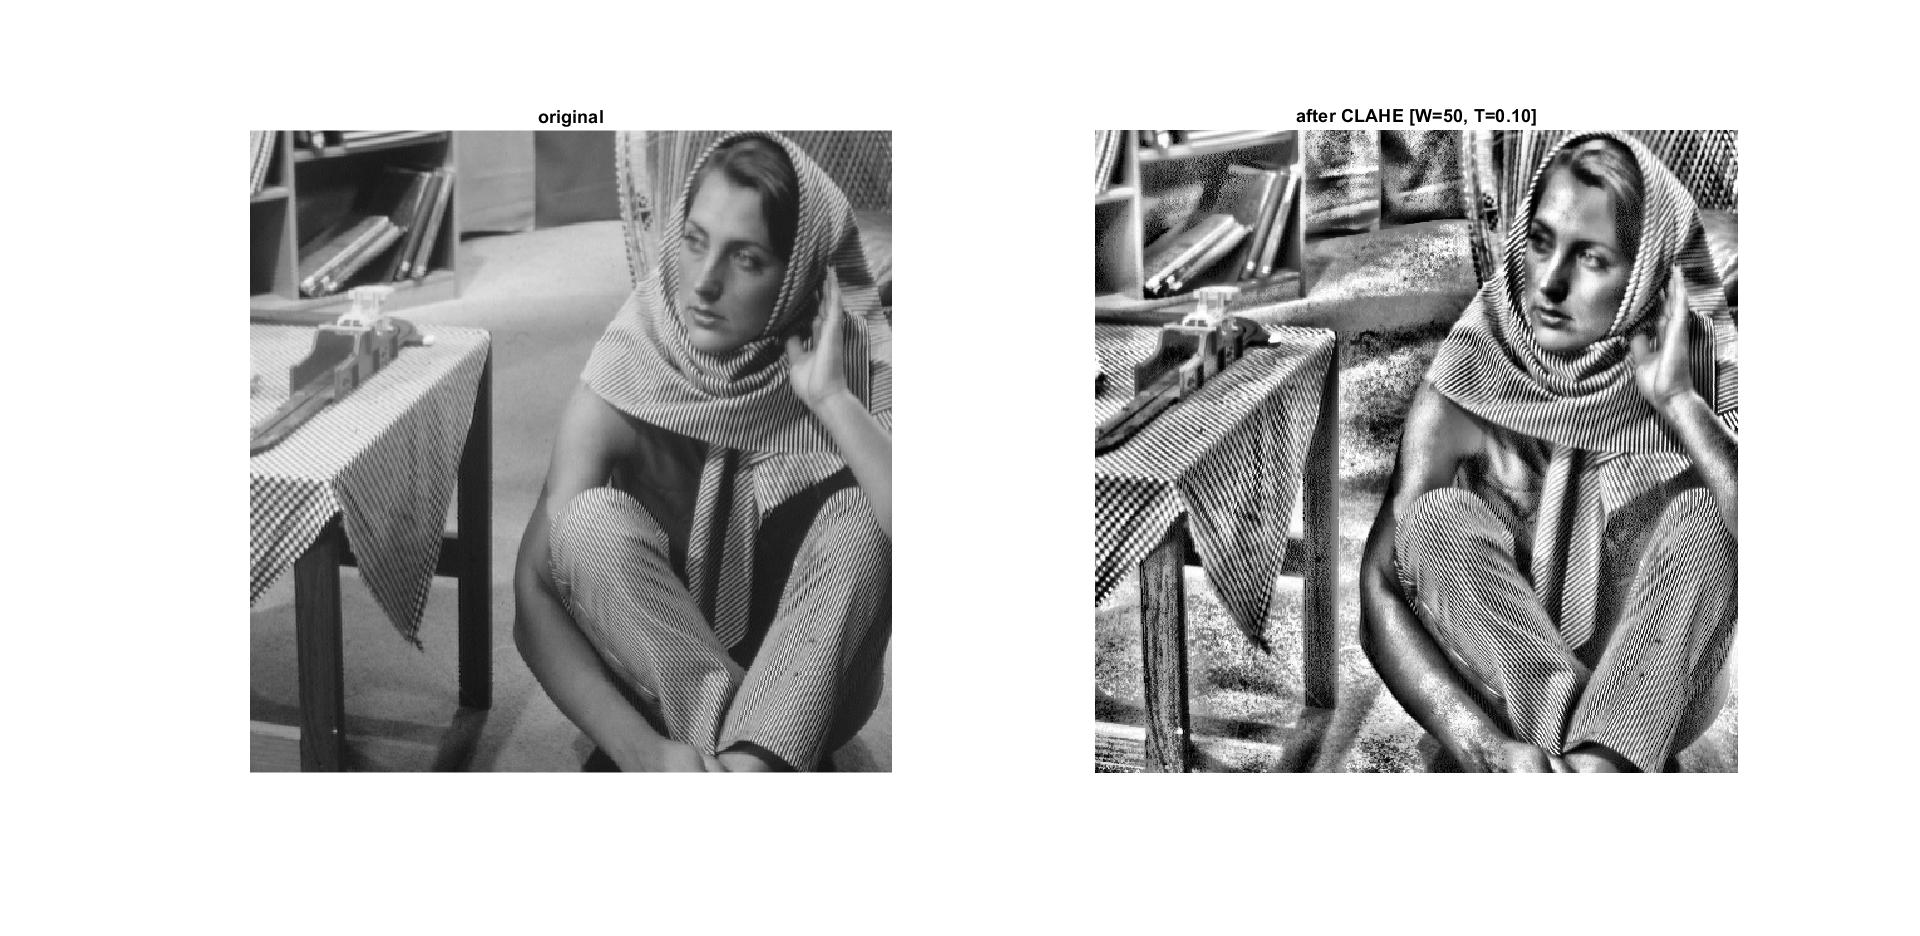
\includegraphics[width=\textwidth]{e11.jpg}
    \vspace*{-55pt}
    \caption{Transformation 1 on Image(1)}
    \label{fig:5.11}
\end{figure}
\renewcommand{\thefigure}{5.12}
\begin{figure}[H]
    \centering
    \vspace*{-30pt}
    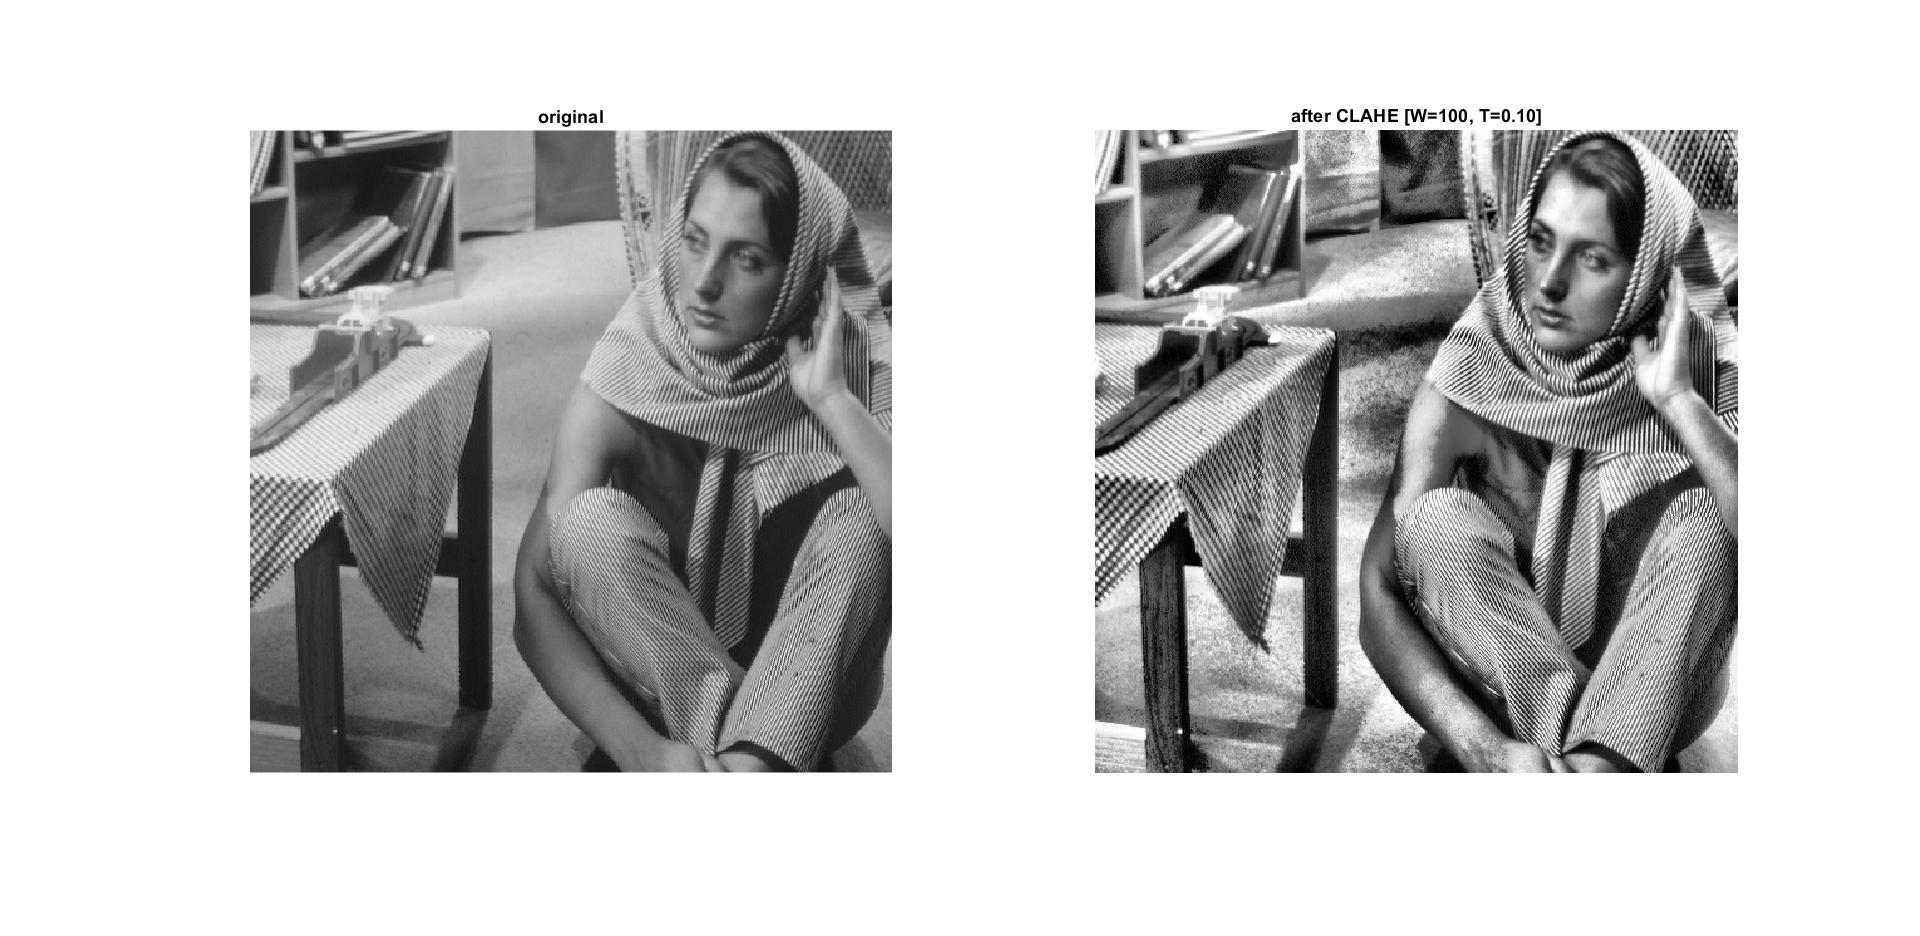
\includegraphics[width=\textwidth]{e12.jpg}
    \vspace*{-55pt}
    \caption{Transformation 2 on Image(1)}
    \label{fig:5.12}
\end{figure}
\renewcommand{\thefigure}{5.13}
\begin{figure}[H]
    \centering
    \vspace*{-30pt}
    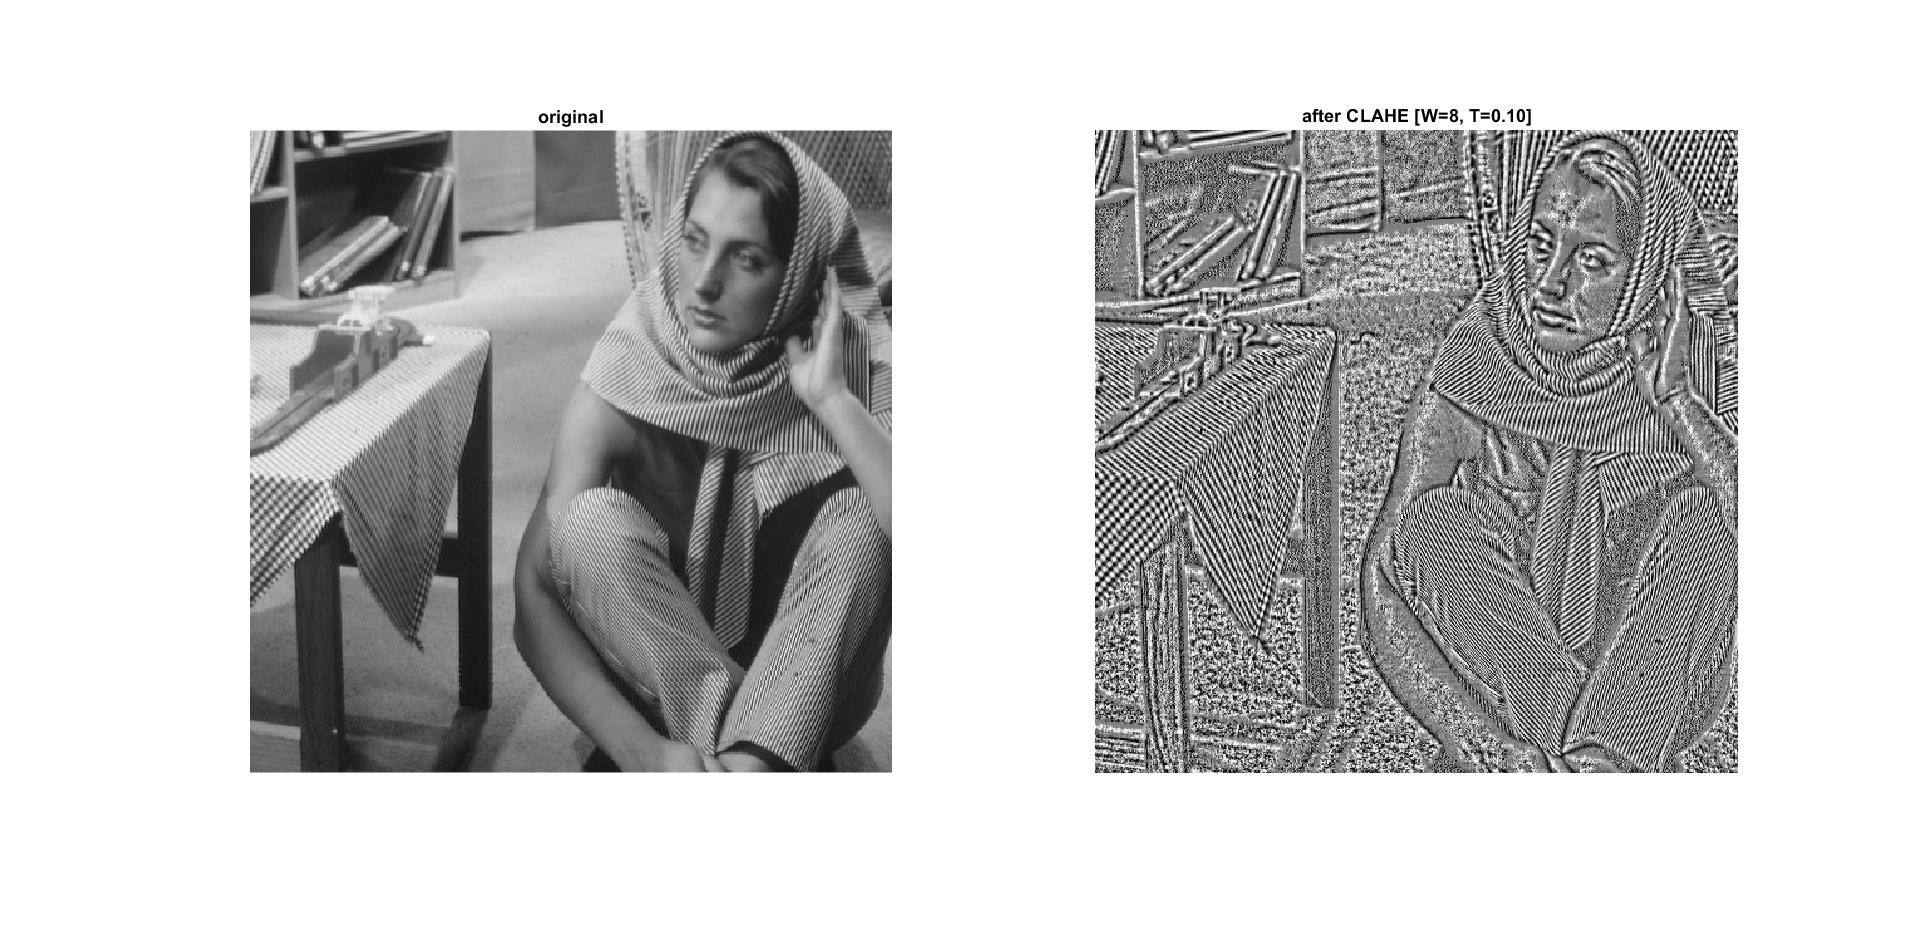
\includegraphics[width=\textwidth]{e13.jpg}
    \vspace*{-55pt}
    \caption{Transformation 3 on Image(1)}
    \label{fig:5.13}
\end{figure}
\renewcommand{\thefigure}{5.14}
\begin{figure}[H]
    \centering
%    \vspace*{-30pt}
    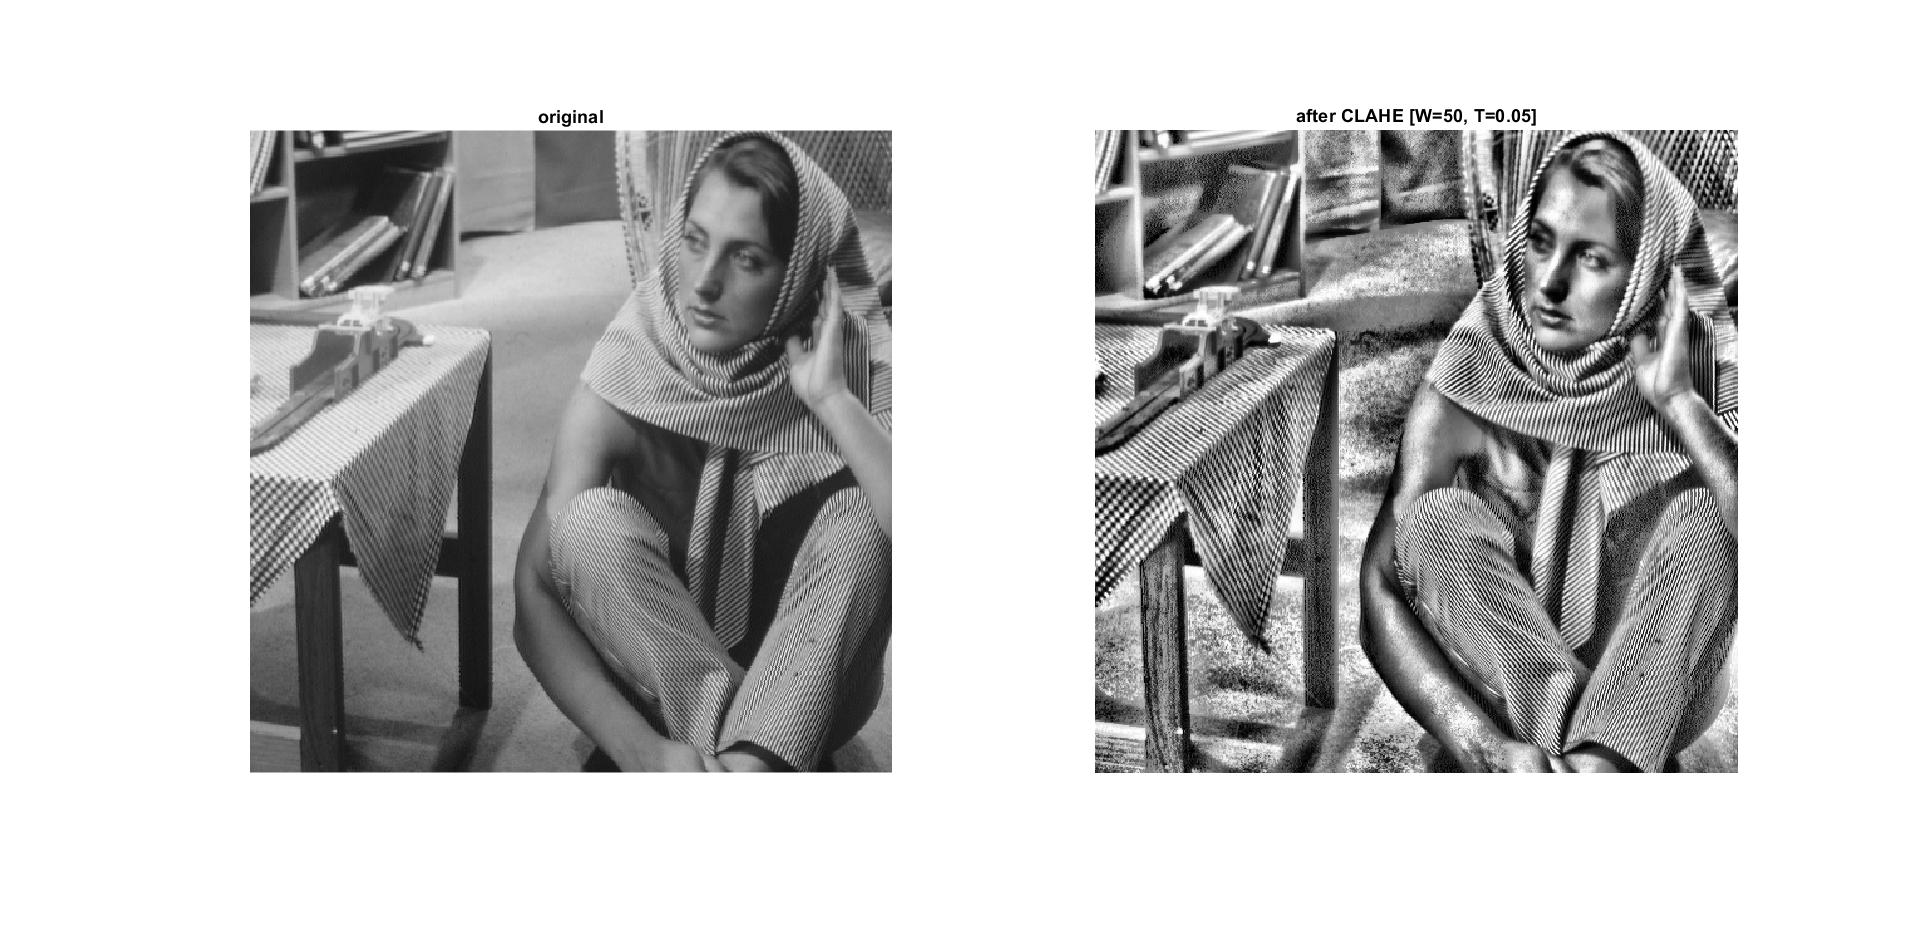
\includegraphics[width=\textwidth]{e14.jpg}
    \vspace*{-55pt}
    \caption{Transformation 4 on Image(1)}
    \label{fig:5.14}
\end{figure}

\renewcommand{\thefigure}{5.21}
\begin{figure}[H]
    \centering
    \vspace*{-30pt}
    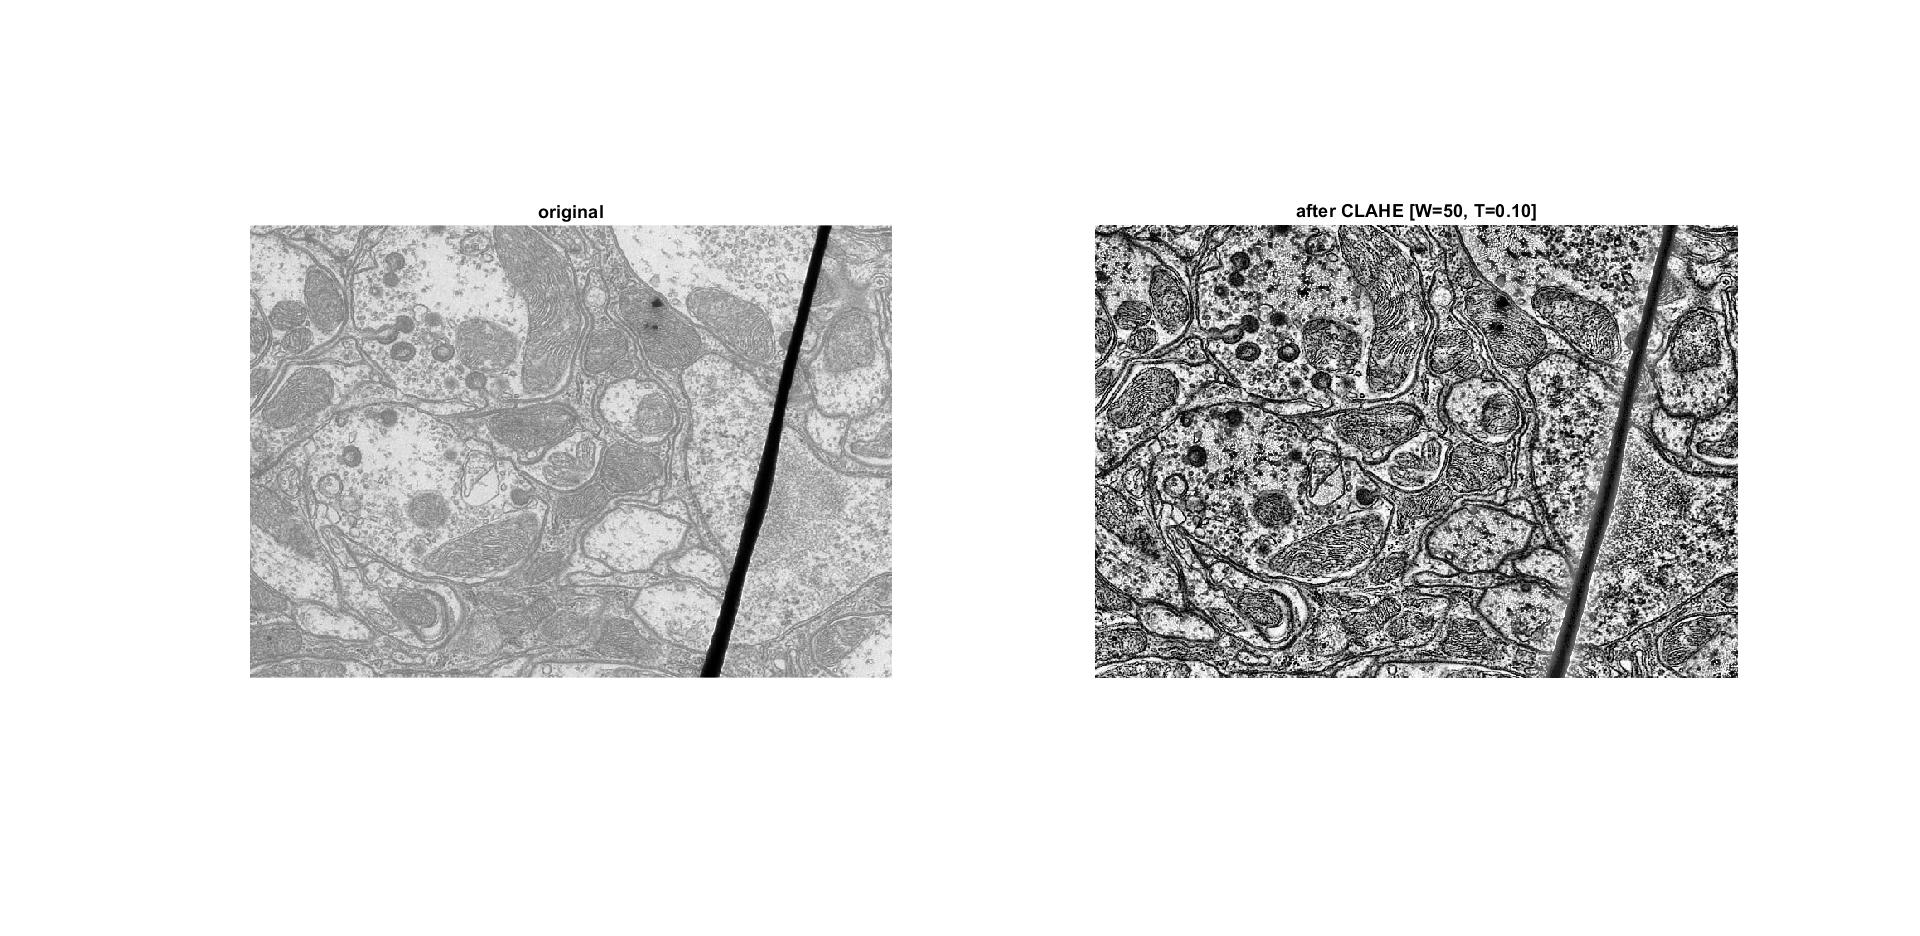
\includegraphics[width=\textwidth]{e21.jpg}
    \vspace*{-80pt}
    \caption{Transformation 1 on Image(2)}
    \label{fig:5.21}
\end{figure}
\renewcommand{\thefigure}{5.22}
\begin{figure}[H]
    \centering
    \vspace*{-30pt}
    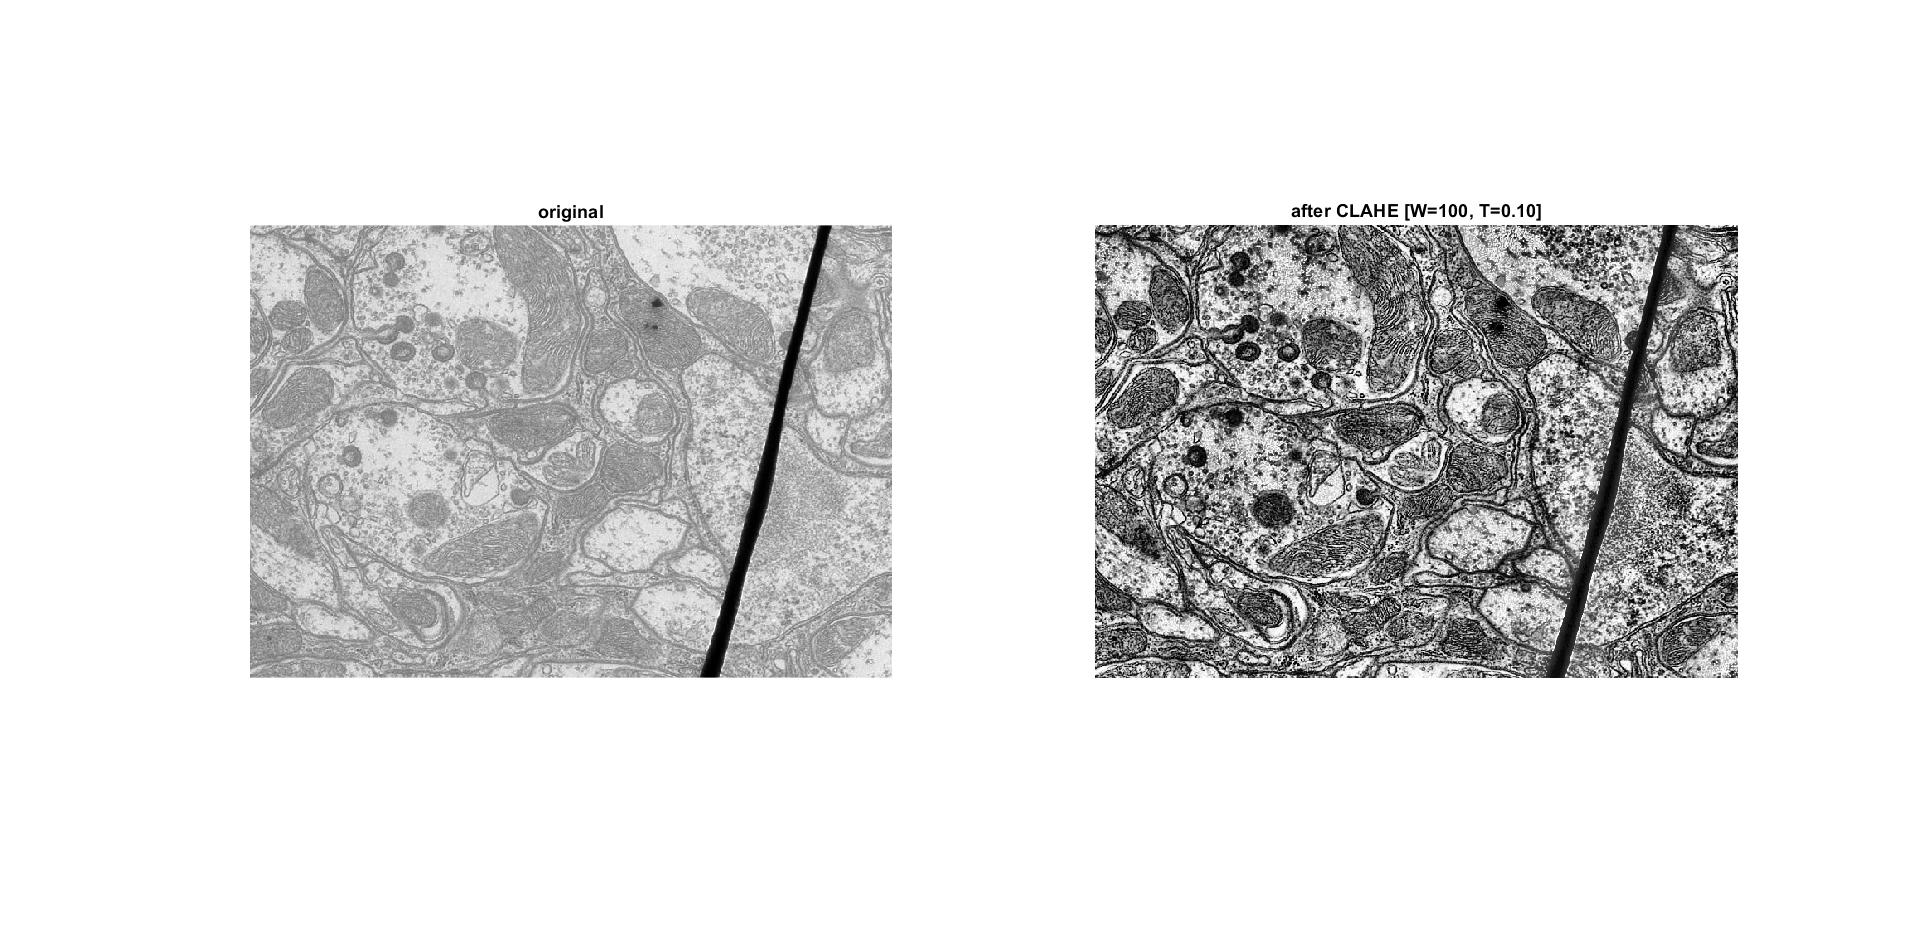
\includegraphics[width=\textwidth]{e22.jpg}
    \vspace*{-80pt}
    \caption{Transformation 2 on Image(2)}
    \label{fig:5.22}
\end{figure}
\renewcommand{\thefigure}{5.23}
\begin{figure}[H]
    \centering
%    \vspace*{-30pt}
    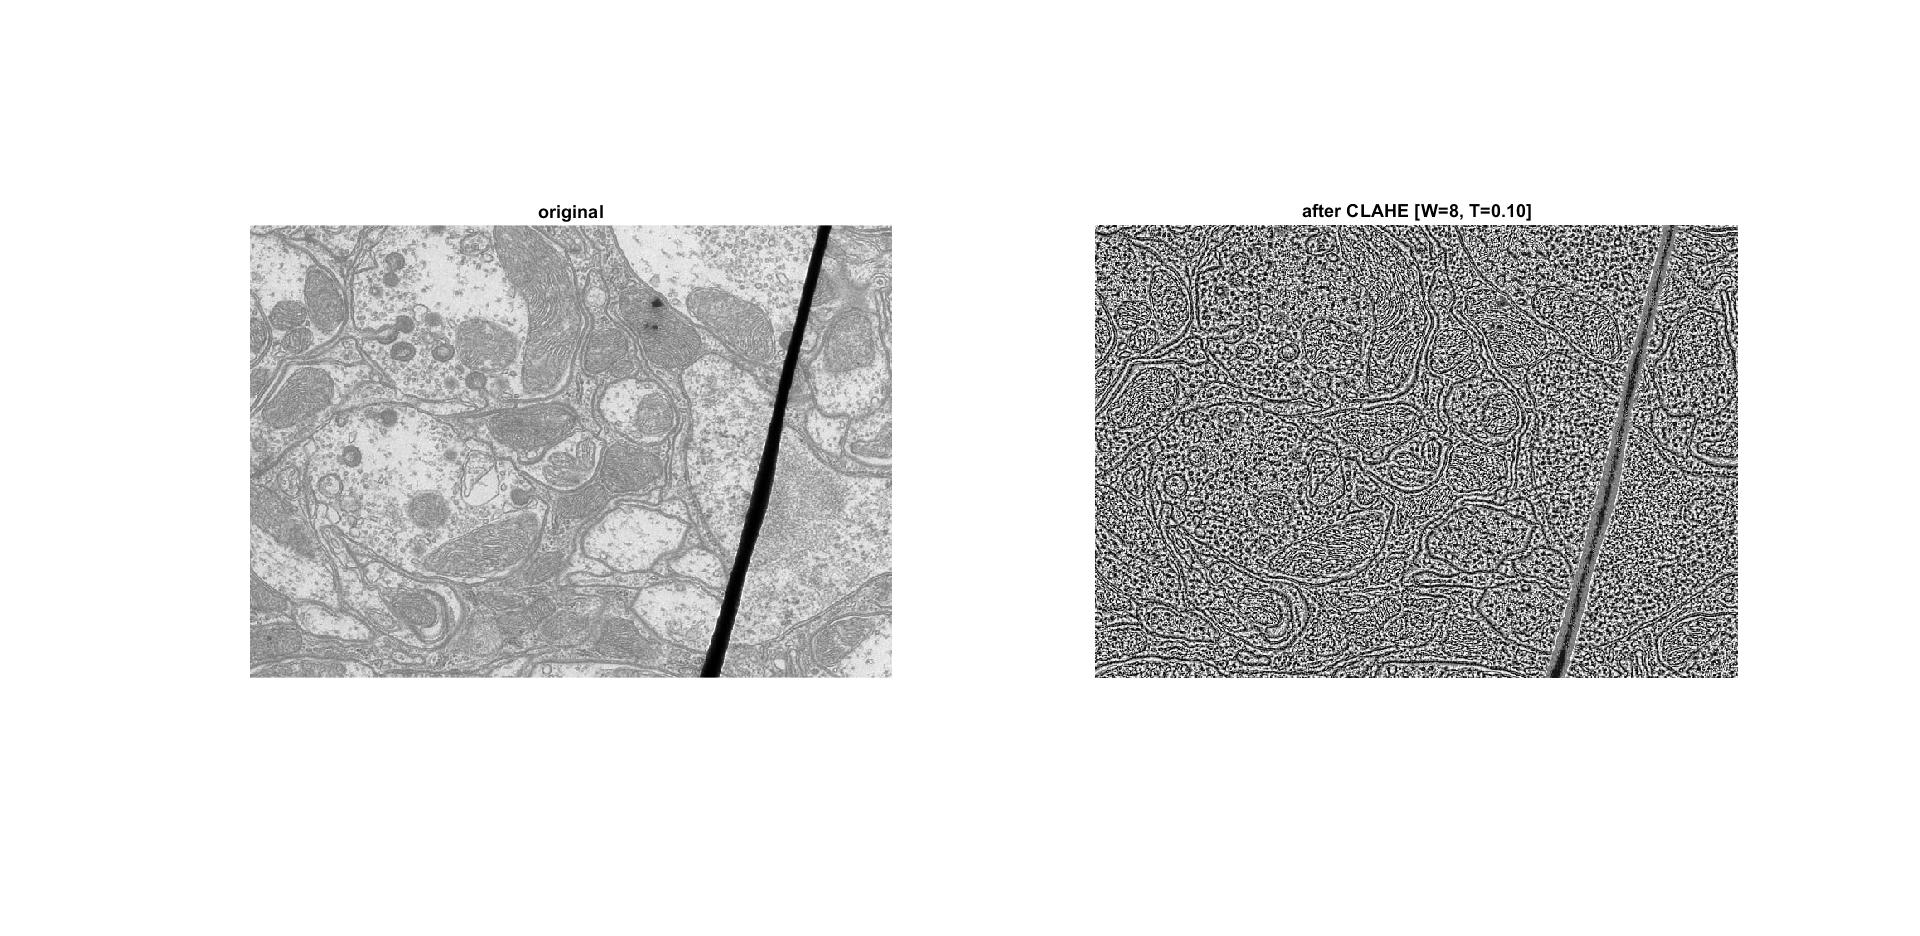
\includegraphics[width=\textwidth]{e23.jpg}
    \vspace*{-80pt}
    \caption{Transformation 3 on Image(2)}
    \label{fig:5.23}
\end{figure}
\renewcommand{\thefigure}{5.24}
\begin{figure}[H]
    \centering
    \vspace*{-30pt}
    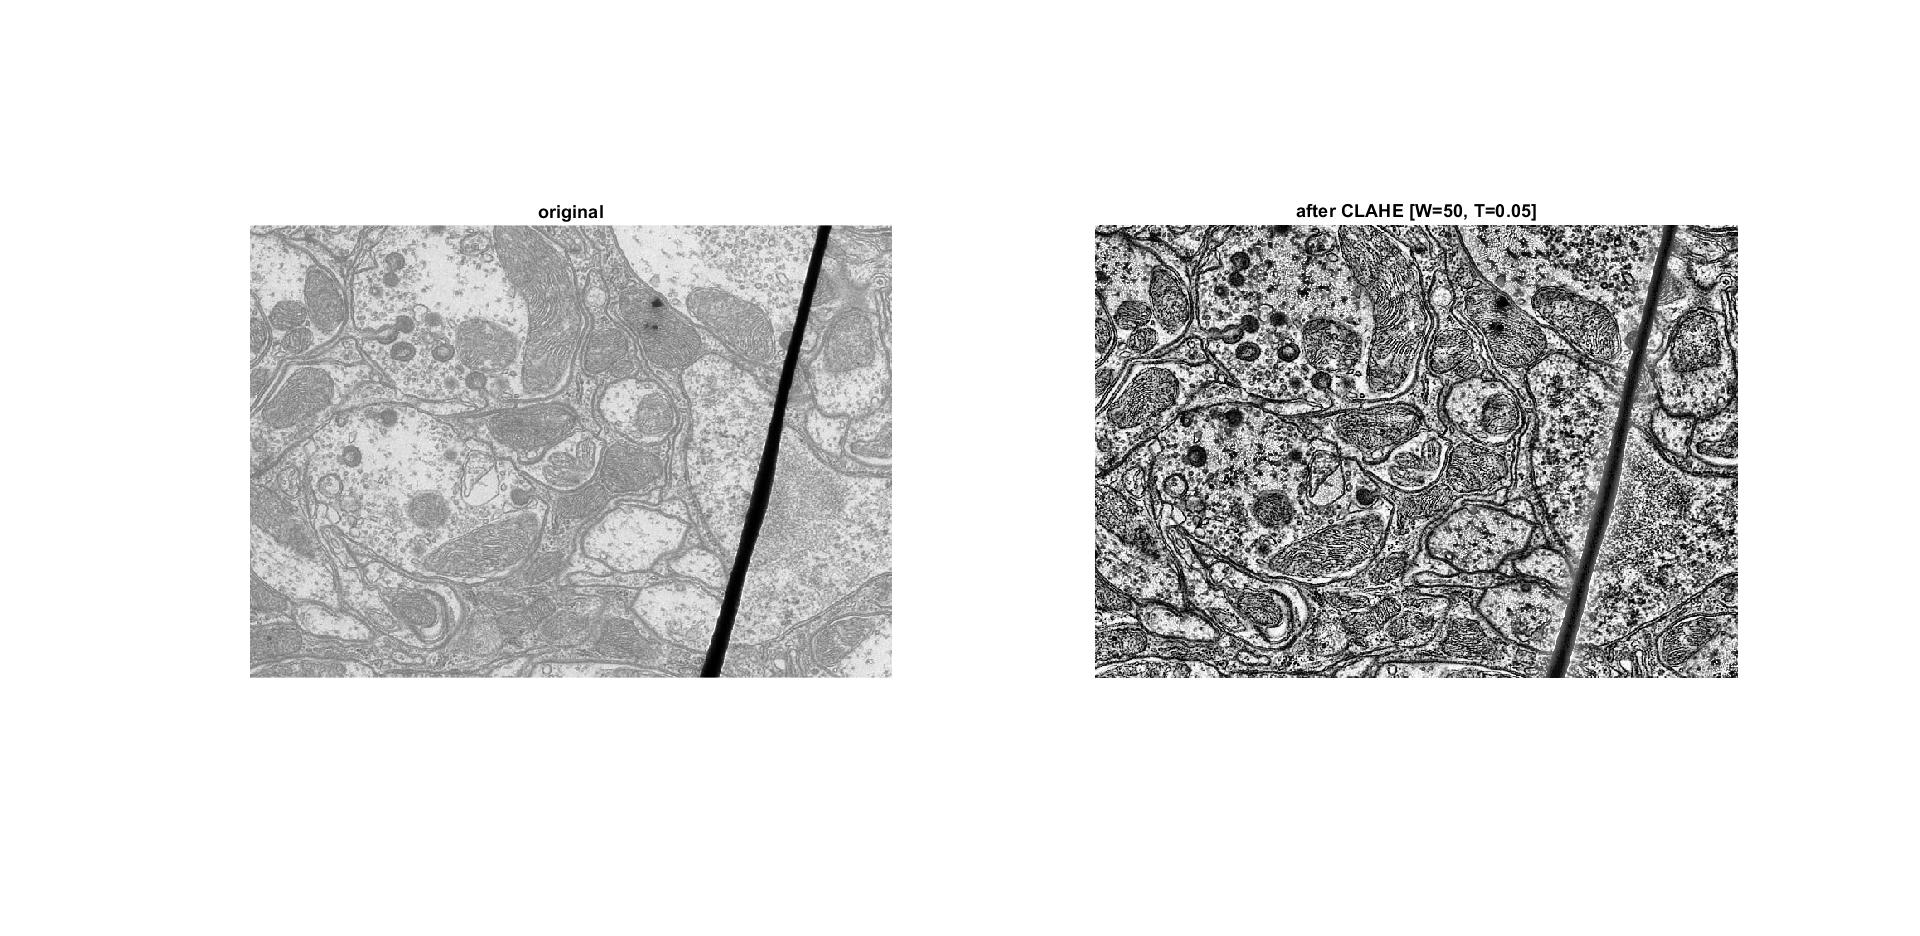
\includegraphics[width=\textwidth]{e24.jpg}
    \vspace*{-80pt}
    \caption{Transformation 4 on Image(2)}
    \label{fig:5.24}
\end{figure}

\renewcommand{\thefigure}{5.31}
\begin{figure}[H]
    \centering
    \vspace*{-30pt}
    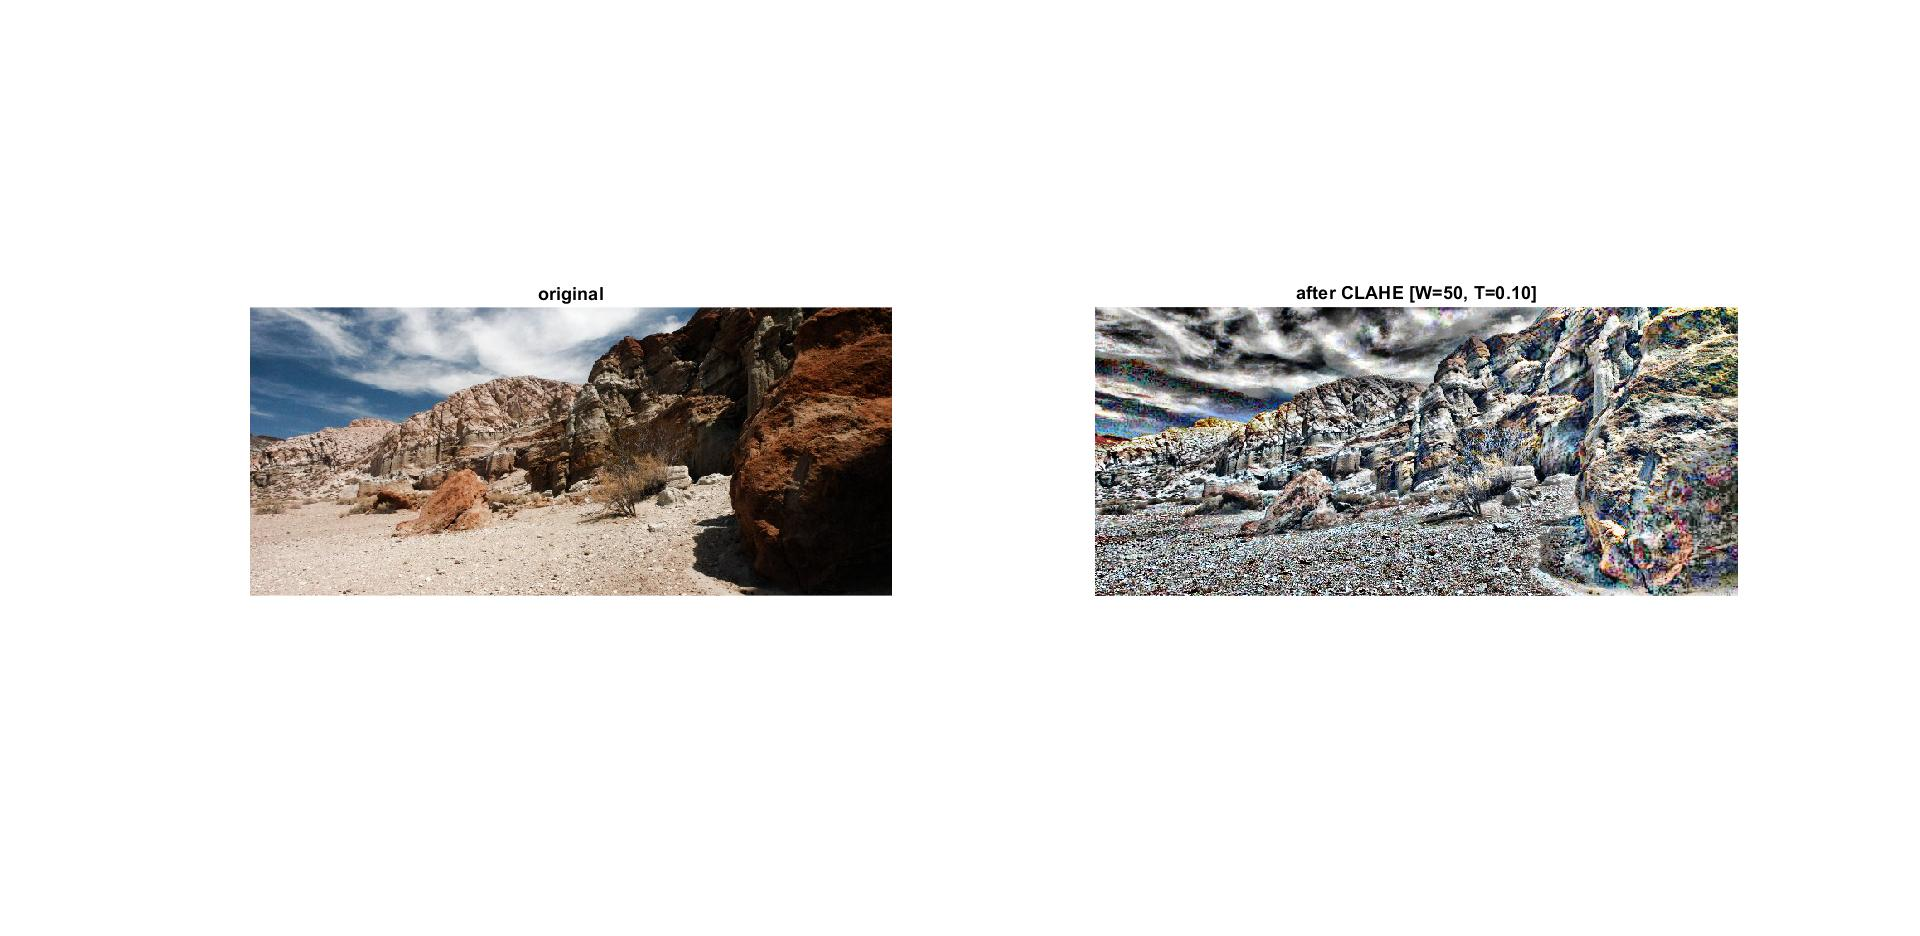
\includegraphics[width=\textwidth]{e31.jpg}
    \vspace*{-90pt}
    \caption{Transformation 1 on Image(3)}
    \label{fig:5.31}
\end{figure}
\newpage
\renewcommand{\thefigure}{5.32}
\begin{figure}[H]
    \centering
%    \vspace*{-30pt}
    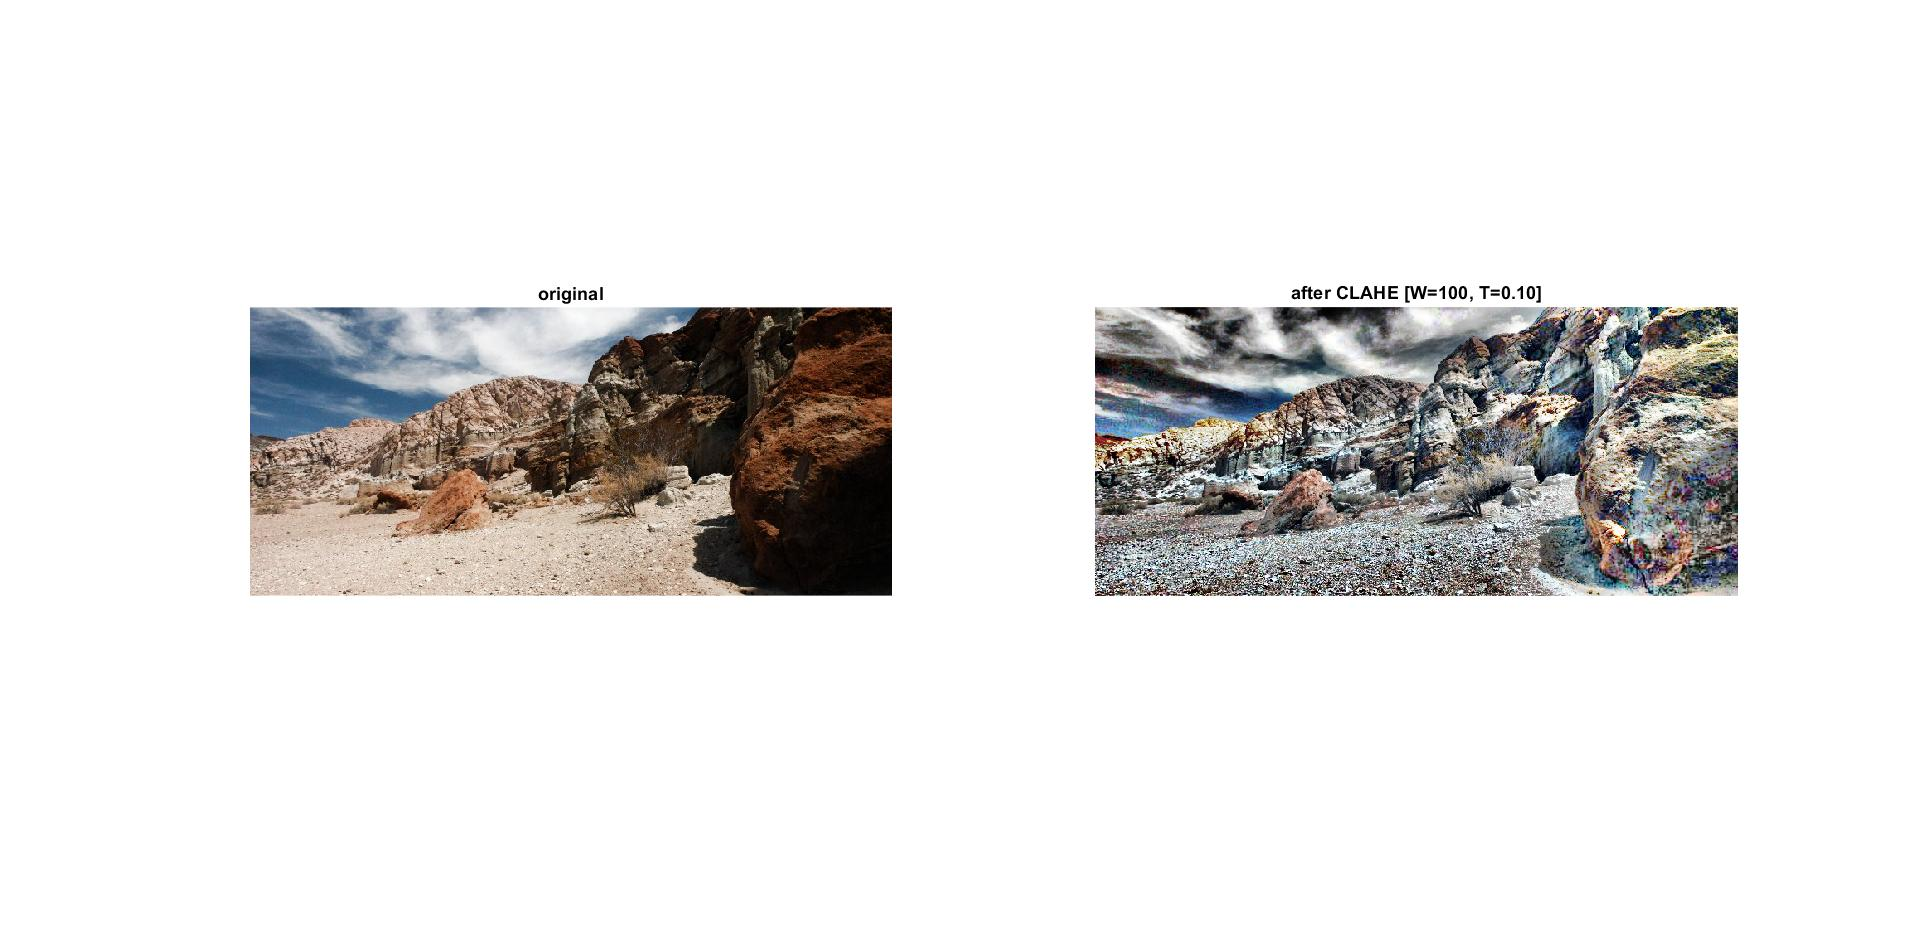
\includegraphics[width=\textwidth]{e32.jpg}
    \vspace*{-90pt}
    \caption{Transformation 2 on Image(3)}
    \label{fig:5.32}
\end{figure}
\renewcommand{\thefigure}{5.33}
\begin{figure}[H]
    \centering
    \vspace*{-30pt}
    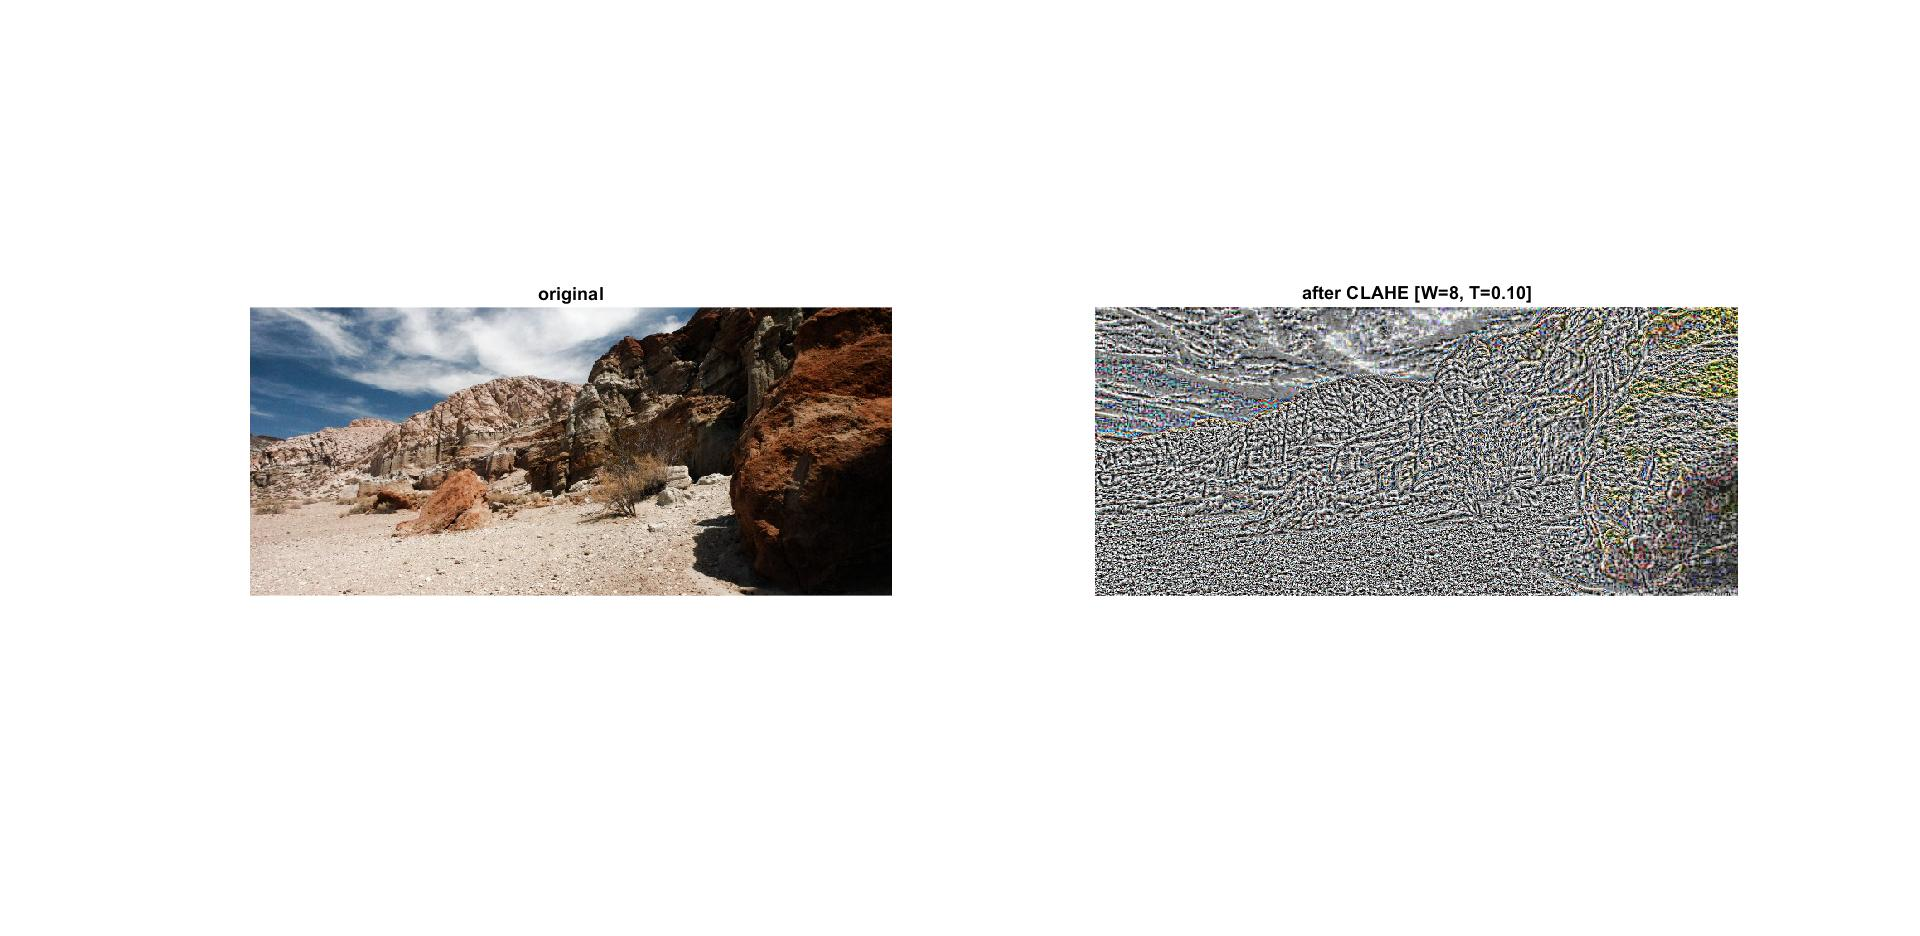
\includegraphics[width=\textwidth]{e33.jpg}
    \vspace*{-90pt}
    \caption{Transformation 3 on Image(3)}
    \label{fig:5.33}
\end{figure}
\renewcommand{\thefigure}{5.34}
\begin{figure}[H]
    \centering
    \vspace*{-30pt}
    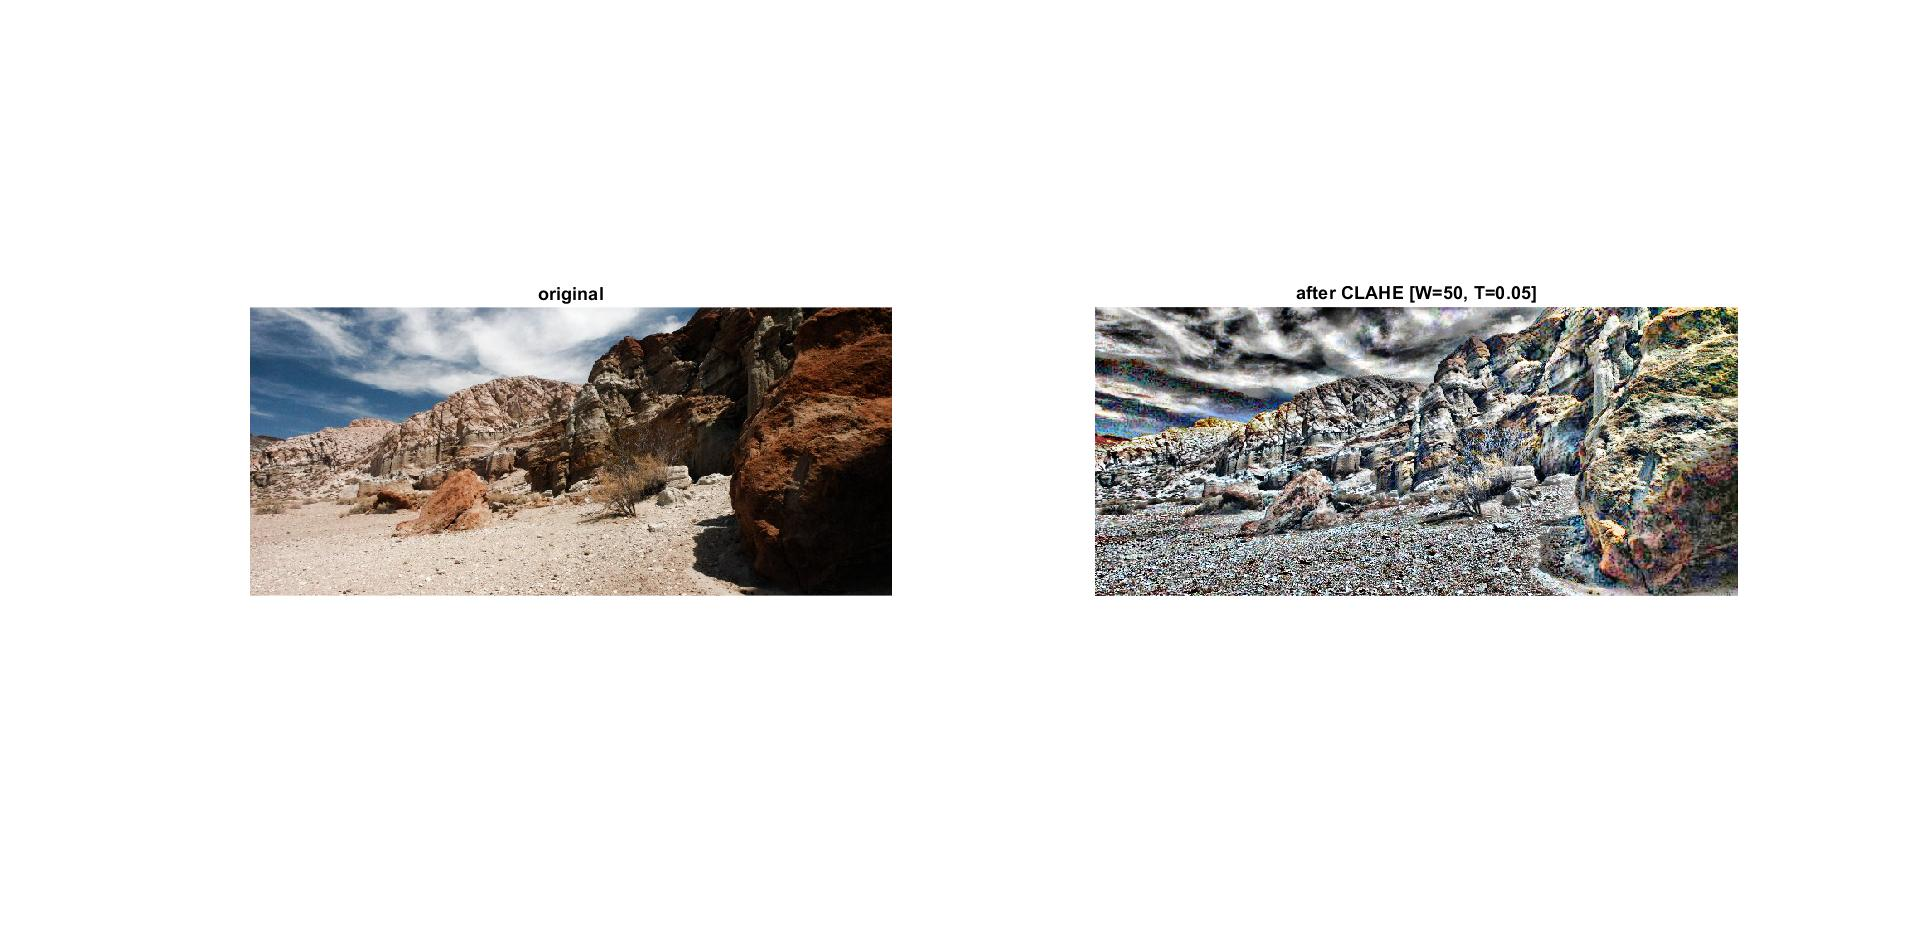
\includegraphics[width=\textwidth]{e34.jpg}
    \vspace*{-90pt}
    \caption{Transformation 4 on Image(3)}
    \label{fig:5.34}
\end{figure}
\newpage
\renewcommand{\thefigure}{5.61}
\begin{figure}[H]
    \centering
%    \vspace*{-30pt}
    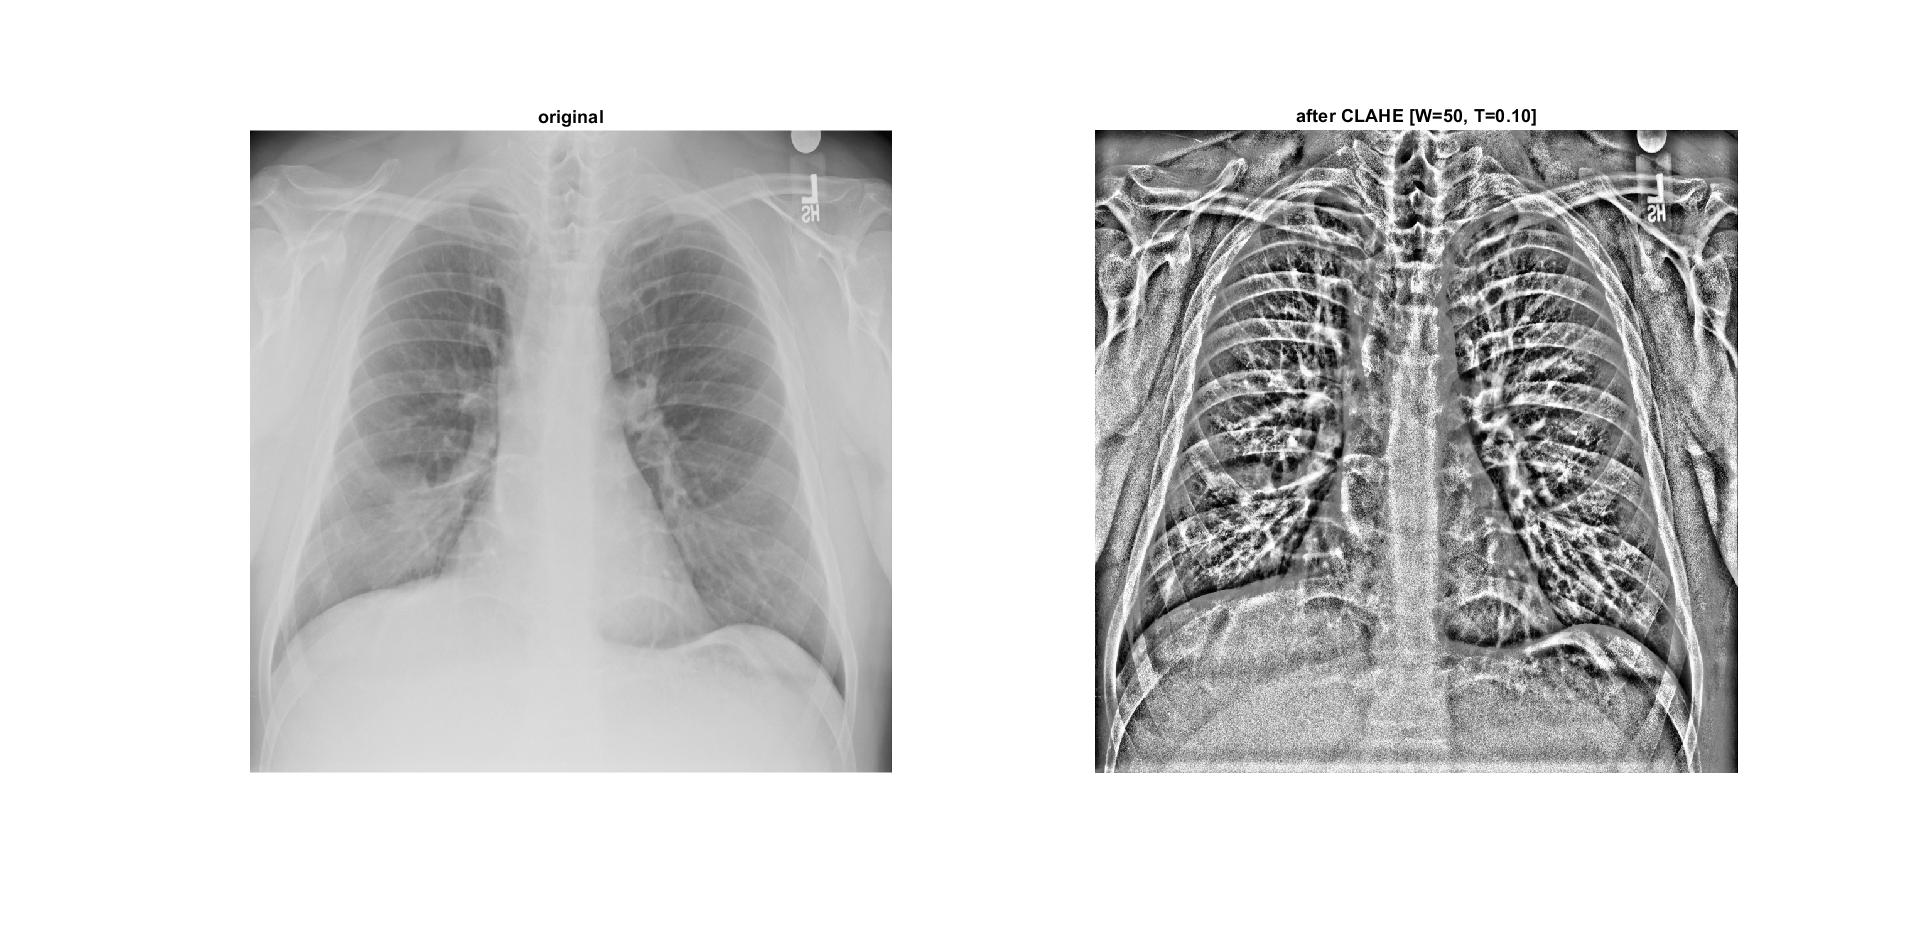
\includegraphics[width=\textwidth]{e61.jpg}
    \vspace*{-60pt}
    \caption{Transformation 1 on Image(6)}
    \label{fig:5.61}
\end{figure}
\renewcommand{\thefigure}{5.62}
\begin{figure}[H]
    \centering
    \vspace*{-30pt}
    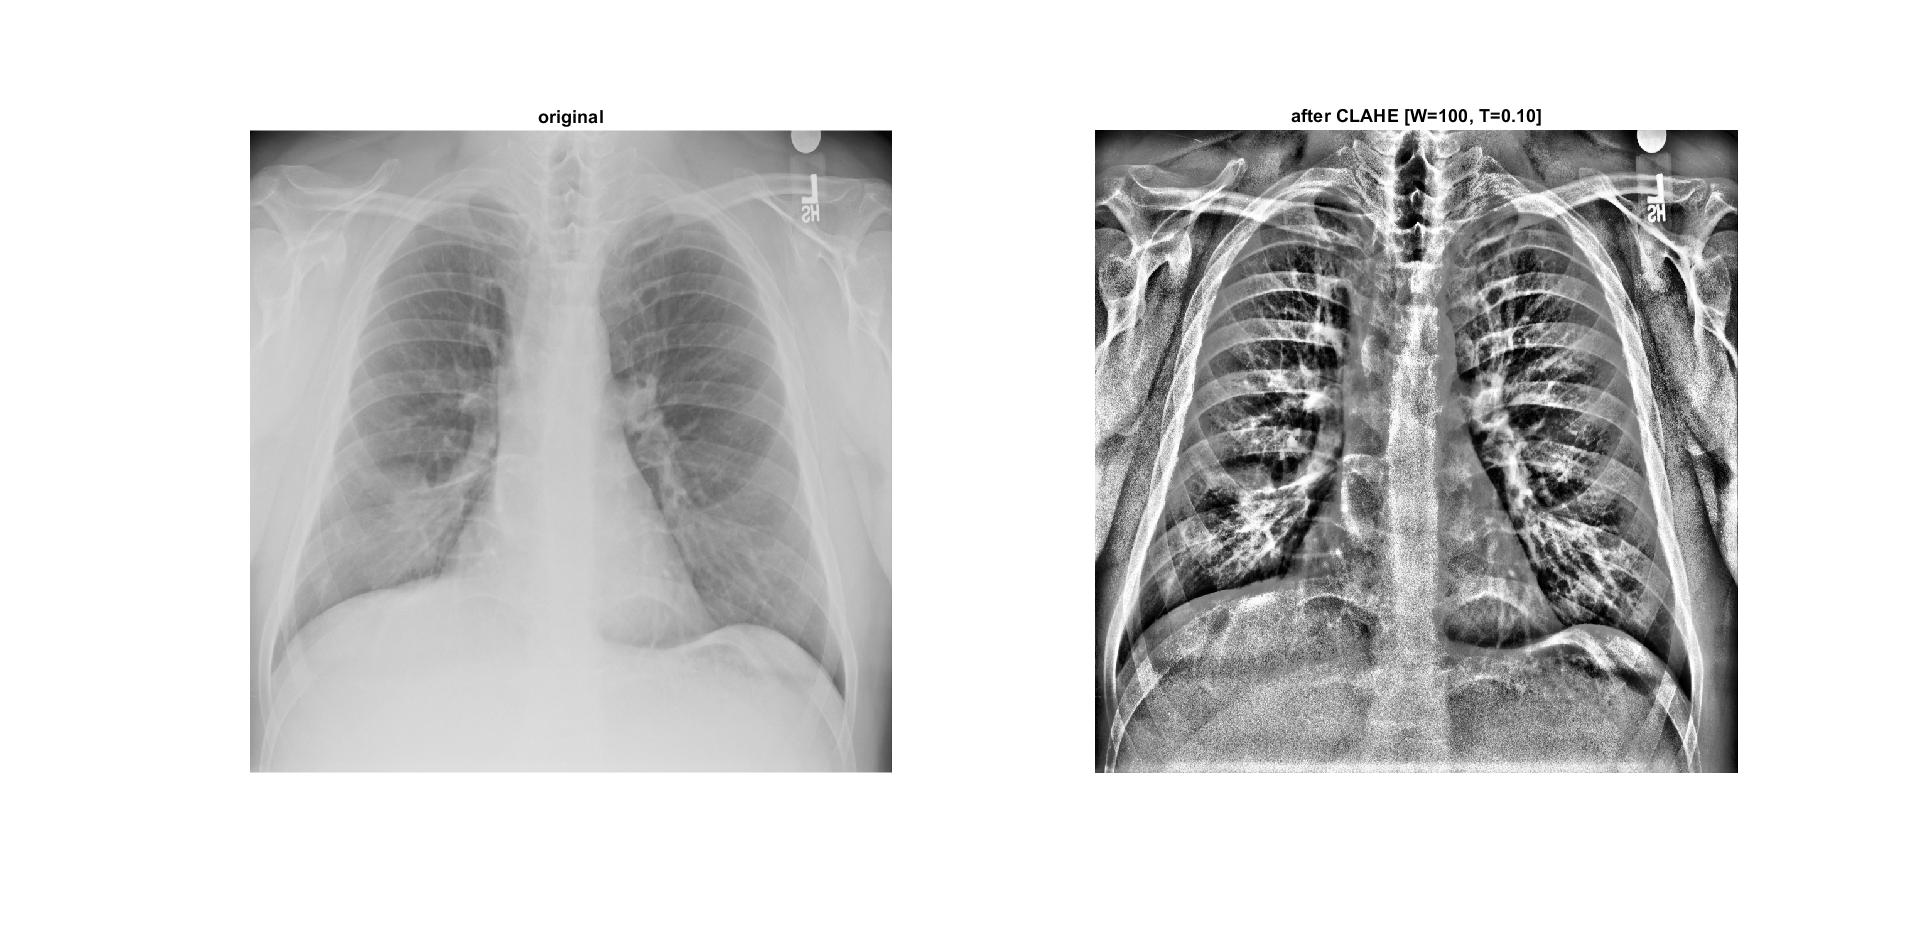
\includegraphics[width=\textwidth]{e62.jpg}
    \vspace*{-60pt}
    \caption{Transformation 2 on Image(6)}
    \label{fig:5.62}
\end{figure}
\renewcommand{\thefigure}{5.63}
\begin{figure}[H]
    \centering
    \vspace*{-30pt}
    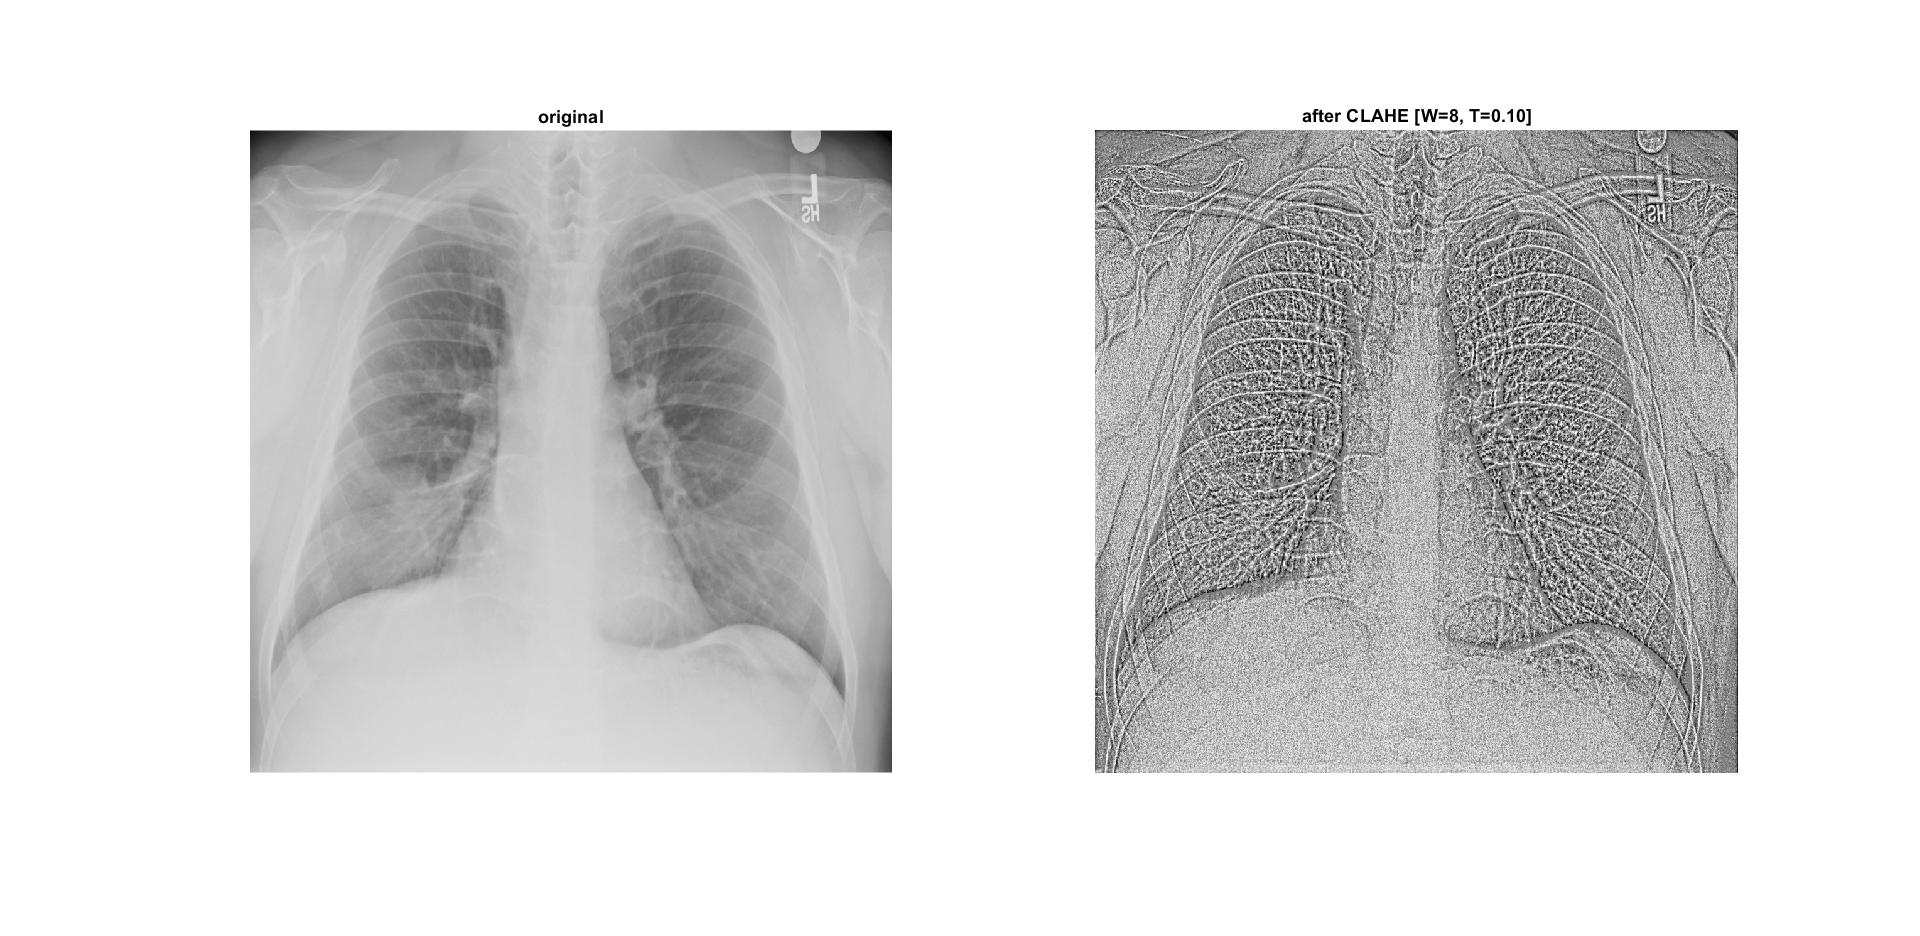
\includegraphics[width=\textwidth]{e63.jpg}
    \vspace*{-60pt}
    \caption{Transformation 3 on Image(6)}
    \label{fig:5.63}
\end{figure}
\renewcommand{\thefigure}{5.64}
\begin{figure}[H]
    \centering
%    \vspace*{-30pt}
    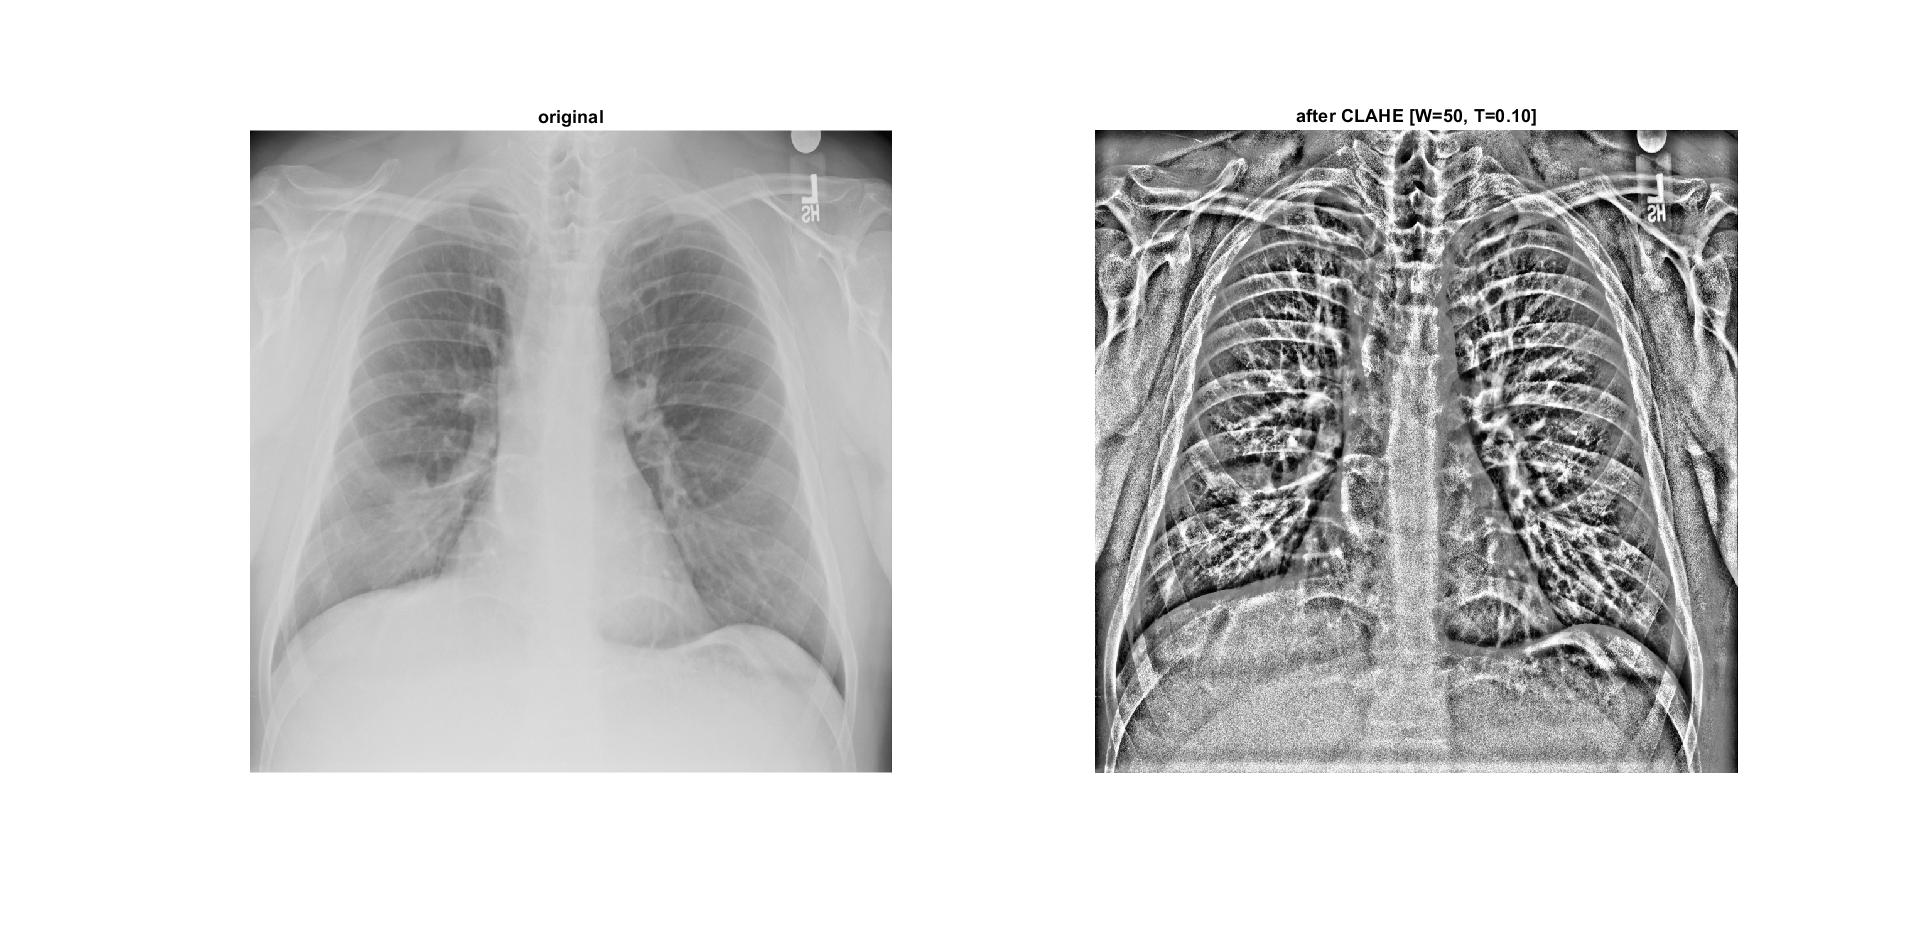
\includegraphics[width=\textwidth]{e64.jpg}
    \vspace*{-60pt}
    \caption{Transformation 4 on Image(6)}
    \label{fig:5.64}
\end{figure}

\end{document}